% !TeX root = ../main.tex

\chapter{整数快速卷积实现}
\label{cha:chapter03}

\section{Winograd卷积实现简介}

Winograd 卷积的一般过程包括输入变换(input transform),权重变换(weight transform),矩阵乘法(GEMM)以及输出变换(output transform)。
其中权重的变换只用操作一次,便可以在不同的输入复用。一般考虑到运行时效率,权重变换可以在卷积操作实际执行前操作,从而Winograd 卷积的实际执行过程可以概况为
以下步骤:
\begin{enumerate}
  \item 将输入的图像块转换到 Winograd 域
  \item 执行在 Winograd 域中执行变换后的输入和权重的矩阵乘法
  \item 将矩阵乘法的结果转换回空间域
\end{enumerate}

若使用$F(m, r)$ 
 \footnote{下面对于卷积实现中的一些符号做如下约定。卷积操作作用于输入特征的局部,并且局部特征的卷积结果输出也仅由这一局部的输入所决定。对于输入局部(input tile)尺寸位 $m x m $,
 卷积核(kernel)尺寸为 $k x k$ ,输出块(output tile)特征大小为 $ r x r $ 的卷积操作,可以记为 $ F(r\times r, k\times k, m\times m) $ .}
有m个输出的r-tap FIR滤波器,F(m, r) 接收的输入的大小为 ( m + r - 1), 则 Winograd 卷积算法可以表示为

\begin{align}
\label{eq:winograd1d}
  Y = A^T [(Gg) \circ (B^Td)]
\end{align}

在式 \ref{eq:winograd1d} 中,$\circ$ 表示 Hadamard Product.

Winograd 卷积算法中的矩阵乘法量同输入的尺寸一致,即 $F(m, r)$ 的Winograd 卷积,其中需要执行 m + r -1 个乘法。而更高维度的Winograd 算法 $F(mxn, rxs)$,则可以通过
在对应的 维度嵌套一维的卷积算法\ref{eq:winograd1d} $F(m, r)$ 和 $F(n, s)$ 实现。特别是对于卷积网络中,最为广泛使用的方形滤波器,即卷积核的宽高相等,$F(m x m, r x r)$
表示卷积核尺寸为 $r x r$,对应的输出尺寸为 $ m x m$, 二维的 Winograd 算法可以表示为 :

\begin{align}
\label{eq:winograd2d}
  Y = A^T [(GgG^T) \circ (B^TdB)] A
\end{align}

而与之对应的直接卷积方法中对应的矩阵乘法则为 $m^2r^2$ (输出为$m^2$个,每个输出对应着$r^2$个输入,每个输入都要同filter中的对应值做一次乘法),而这里二维场景的
Winograd卷积实现,其中的乘法操作的规模为 $( m + r - 1)^2$。而在卷积算法的实现中,矩阵乘法(GEMM)无疑是最为占据主导的操作,自然也是效率优化的瓶颈。于是,以乘法的
规模作为复杂度的度量,Winograd 卷积相对于直接卷积方法,实现的复杂度简化为

\begin{align}
  \label{eq:winograd_reduction}
  \frac{m^2r^2}{(m+r-1)^2}
\end{align}

因此,对于较为常用的两类Winograd 卷积实现 F(2, 3), F(4, 3),即卷积核大小均为3,输出的尺寸分别为2和4的卷积,理论上分别可以达到2.25 和 4倍的加速。而在实际的实现中,
还需要考虑到对于输入和输出的变换所带来的额外开销,在卷积的规模,特别是矩阵乘法的规模没有达到一定的限度时,Winograd卷积方法不一定能够实现理论的加速值。
尽管使用更大尺度(输出的尺度和卷积尺度)的Winograd 卷积可以实现更大程度的复杂度简化,但同时也受限于变换过程的数值稳定性,更大尺度的 Winograd 卷积一般也
意味着不准确,可能会存在精度的损失。

另外,关于Winograd 卷积中使用的变换矩阵 $G$, $B^T$, $A^T$ 的具体表示的推导可以通过Cook Toom 算法来实现。具体过程可以概述为,使用拉格朗日插值多项式,将相当于卷积
的多项式乘法,转换为多项式在固定数目的插值点处取值的逐元素乘法。 Cook-Toom算法的缺点是,随着变换大小的增加,变换很快变得不稳定。 但是,它们非常适合卷积神经网络中使用的3x3小卷积。

Winograd快速卷积算法的更一般形式是使用中国剩余定理。 Cook Toom 算法只是其中之一。而这一过程的具体不在本文的范畴,有兴趣的可以参考工作\cite{Lavin2015FastAF} 中的补充材料。


快速卷积算法相对于直接卷积和基于GEMM的卷积(比如im2col,im2row等)的实现的主要一大优化目标在于减小运算中乘法的规模,尽管快速卷积方法往往为实现减少乘法的数目而不惜引入
一些额外的加法操作以及对于输入的变换,但在运算中乘法操作达到一定的规模后,乘法数目减少所带来的计算收益是可以超过这些额外的开销的。值得注意的是,快速卷积方法中为减少乘法
操作而不惜引入加法的这一优化手段,并不是因为加法操作会比乘法操作快,这个概念具体到现代的硬件设备上的乘法和加法实现实际上是不合理的。而且实际上在现代硬件设备中
乘法和加法操作往往是可以聚合(fused)在一起的,也就是乘累加(multiply and acculate)操作。从而即使额外引入加法,在仔细设计算法执行后,是不会带来 额外的计算开销的。另外,通过充分利用FMA实现计算加速,在算法设计中添加加法来减少乘法,需要考虑到计算中的乘法和加法的平衡,加法操作需要同乘法操作匹配,否则,额外的加法会
带来计算负担,甚至会超过乘法减少和FMA换取的计算量的减少值,从而反而使得计算变得低效。

而另外一方面,作为另外一种更为常用的快速卷积方法实现,快速傅里叶变换(FFT)方法在整体的形式上同Winograd 方法\ref{eq:winograd1d}类似,
其中的变换过程则会对应为FFT和inverse 类似,其中的变换过程则会对应为FFT和inverse
 FFT,即变换矩阵$G$ 和 $B^T$表示FFT,而$A^T$ 则表示inverse FFT。同时,式\ref{eq:winograd1d} 中的也将对应的修改为复数乘法,同实数乘法不同的是,直接的复数乘法需要
 4 次实数乘法来实现。然而,卷积网络中的输入往往都是实数,而实数的傅里叶变换存在Hermitian对称性,从而可以将矩阵复数乘法的复杂度减半,只需计算矩阵中的一半的值,另外一半
 只需要取对应的已计算值的共轭复数即可。但即便如此,FFT卷积实现中仍然需要达到 64x64 的输入尺度才能在乘法规模的优化程度上达到和 Winograd 卷积 F(4, 3) 在输入为6x6 时的
 同等水准,使用FFT实现卷积操作的加速需要相比于Winograd卷积更大的内存需求,


\section{Winograd 算法数值稳定性}

尽管Winograd 算法是现已知的在计算复杂度而言最优的卷积算法, 然而 Winograd 卷积算法具有着数值
计算不稳定的特质。在卷积的尺度相对比较小(比如$F(2,3)$, $F(4, 3)$),并且参与运算的数值为单精度或
者双精度浮点数时,Winograd 卷积的结果仍然是相当精确的,但是当卷积的尺度变大,或者参数计算的数值
精度降低时,这一情况却不容乐观了。这也限制了Winograd 卷积的适用范围,在卷积核或者卷积操作输入的
子块的尺度较大的情形下,Winograd卷积的精确性便会有比较明显的损失。 Winograd 卷积计算的精确性
可以通过找出更加合适的Winograd 算法的导出式有关,即通过 Toom-Cook 算法或者CRP理论选择合适的
插值点导出对应的输入变化,权重变换和输出变换矩阵。 这里需要说明的一点是,Winograd 
卷积的数值不稳定性,带来的只是一种边际数值误差(marginal error),因此,Winograd 卷积在很多情形
下只是应用于模型 的推理阶段,
即网络在训练的过程中使用常规的卷积算法,而在模型前向推理的过程中,是完全可以将对应的满足条件的
卷积操作可以替换为 Winograd 卷积算法。

表 \ref{tbl:winograd_acc} 中对比了不同尺度的Winograd 卷积算法在不同精度的数据表示下的准确度及数值
稳定性,这里以直接卷积算法的准确率作为对照,可见对于输出尺度大于2 的 Winograd 卷积在low precision 
的场景下在对应视觉任务上的准确率会大幅下降,而这里指的Winograd 卷积指的是在 \cite{Lavin2015FastAF}
以及附带的Toom Cook 方法代码中所导出Winograd 算法形式。究其原因在于,在Winograd 卷积的输出尺度较大
时, 如\ref{eq:winograd_f43} 可见,在变换矩阵 $A^T, G, B^T$ 中对应的数值的范围会变大,并且注意,在
卷积神经网络中常用的2D 卷积中,将其转换为整数型计算时,权重变换矩阵 G 需要扩大 24 倍,则卷积计算过程
中,至少要保证在 $\pm24^2$ 范围内数据的表示和计算数值精度 。

\begin{table}[]
\centering
\caption{ResNet 18 在不同尺度和不同精度的Winograd 卷积算法下的CIFAR-10 分类准确率}
\begin{tabular}{llll}
\hline
\multicolumn{1}{|l|}{}                 & \multicolumn{1}{l|}{32 bit} & \multicolumn{1}{l|}{16 bit} & \multicolumn{1}{l|}{8 bit} \\ \hline
\multicolumn{1}{|l|}{Direct  Conv}     & \multicolumn{1}{l|}{93.16}  & \multicolumn{1}{l|}{93.60}  & \multicolumn{1}{l|}{93.22} \\ \hline
\multicolumn{1}{|l|}{Winograd F(2, 3)} & \multicolumn{1}{l|}{93.16}  & \multicolumn{1}{l|}{93.48}  & \multicolumn{1}{l|}{93.21} \\ \hline
\multicolumn{1}{|l|}{Winograd F(4, 3)} & \multicolumn{1}{l|}{93.14}  & \multicolumn{1}{l|}{19.25}  & \multicolumn{1}{l|}{17.36} \\ \hline
\multicolumn{1}{|l|}{Winograd F(6, 3)} & \multicolumn{1}{l|}{93.11}  & \multicolumn{1}{l|}{11.41}  & \multicolumn{1}{l|}{10.95} \\ \hline
\end{tabular}
\label{tbl:winograd_acc}
\end{table}
\begin{align}
\label{eq:winograd_f43}
  A^T = 
  \begin{pmatrix}
      1 & 1 & 1 &  1 &  1 &  0\\
      0 & 1 & -1&  2 &  -2&  0\\
      0 & 1 & 1 &  4 &  4 &  0\\
      0 & 1 & -1&  8 &  -8&  1
  \end{pmatrix}
  G = 
  \begin{pmatrix}
    \frac{1}{4} & 0 & 0 \\
    -\frac{1}{6} & -\frac{1}{6} & -\frac{1}{6} \\
    -\frac{1}{6} & \frac{1}{6} & -\frac{1}{6} \\
    \frac{1}{24} & \frac{1}{12} & \frac{1}{6} \\
    \frac{1}{24} & -\frac{1}{12} & \frac{1}{6} \\
    0 & 0 & 1
  \end{pmatrix}\\
  B^T =
  \begin{pmatrix}
    4  & 0 &  -5 & 0  &  1&  0\\
    0  & -4&  -4 & 1  &  1&  0\\
    0  & 4 &  -4 & -1 &  1&  0\\
    0  & -2&  -1 & 2  &  1&  0\\
    0  & 2 &  -1 & -2 &  1&  0\\
    0  & 4 &  0  & -5 &  0&  1
  \end{pmatrix}
\end{align}

由于在数值精度较低的情形下Winograd算法表现出明显的数值不稳定性,导致计算精度下降,进而使得在对应视觉任务上的准确性下降,因此在后续的Winograd 量化卷积实现中,本文主要针对于 F(2,3)卷积的实现。

\section{局部区域化多通道的Winograd的卷积算法}

按照上述的Winograd 算法的流程的描述,针对于输入的特征的每个通道做对应的变换,再将变换后的值分别同对应位置的值做乘法似乎是一种直观的实现方法,这种实现不仅在读取输入的过程中缓存友好,而且只需要有限的矢量寄存器就可以完成变换操作,但是在量化计算的场景下,存在这以下新的特性:
\begin{itemize}
  \item 数值表示的精度降低使得计算过程的吞吐得以提升
  \item 使用定点数实现计算存在这频繁的数值表示的变换
\end{itemize}

首先,相对于单精度浮点数表示而言,量化的数值表示可以在同样长的寄存器中存储更多的数值,这不仅使得计算的吞吐变高,同时也需要重新考虑算法的设计与硬件特性的支持。ARM NEON提供了最大 128 位的SIMD 矢量寄存器,尽管相对服务端与桌面端芯片的矢量寄存器所支持的位长相当有限,但应用于8位量化整数的并行计算仍然是有着充分的计算能力。而在Winograd卷积算法中,各个channel之间的数据的计算也实际上是相互独立的,结合硬件计算支持而言,针对于输入的局部区域在通道维度实现并行化计算实则是更为合理的,这样也避免了在量化计算过程中,数值位长的变换带来的算法设计上的频繁改动。而单通道算法在实现Winograd卷积的量化计算中,还需要针对于变换的过程中实现矢量寄存器中数据的转置操作,以及执行矩阵乘法前对于数据的重新排布,这些向量和矩阵的转置操作都是需要相当大的额外开销的,则资源本就有限的ARM设备上这样的操作应该在算法的设计过程中予以避免。而针对于局部的输入区域的多通道特征,恰好可以避免这些转置操作,完成变换的输入和权重可以直接对应到参与矩阵乘法的16个矩阵中。而在寄存器数量允许的条件下,多通道方法尽可能多的使用了可用的寄存器资源,最大化了计算指令与访存指令的比例,更有效的利用了ARM 处理器流水线,可以有效实现计算的高吞吐。

以下针对多通道维度并行化和空间局部性,从Winograd卷积计算中的数据排布,Winograd变换,卷积计算的空间局部化阐述本文在移动设别的量化计算中对于Winograd 卷积的实现设计。

\subsection{适用于量化计算的灵活数据排布}

卷积网络中常用的数据排布方式(data layout)存在 Channel First 即 NCHW 和 Channel Last 即 NHWC 。而对应的在数据加载的过程中,由于在ARMv8-A 架构下,存在 32 个128位
SIMD 寄存器,因此每个寄存器可以用来存储 4 个32位整数(int32)或者 16 个8位整数(uint8)或者 8个16位整数(int16)。以32位整数举例,在NCHW 数据排布下,在完成128位的
数据加载后,一个SIMD 寄存器可以用来储存矩阵中一行的四个值,而在NHWC 数据排布下,同样的单个SIMD寄存器可以用来加载矩阵中位于同一个位置的连续四个通道(channel )的值。
而在Winograd 快速卷积的实现中,NHWC 的数据表示是具备着实现灵活性上的相当的优势的,特别是在量化计算的场景下,定点(fixed point)表示的数据在计算过程中会频繁涉及数据
位长(data width)或者说数据精度(precision)的变换,NHWC的表示可以灵活的实现并行算法。同时在考虑不同规模的算法下,NHWC的data layout 也可以实现寄存器的高效利用。
下面在具体的Winograd 卷积的实现中会做对比和具体的说明。

\subsection{多channel Winograd变换及逆变换}

对于卷积操作$F(2x2, 3x3, 4x4)$, Winograd 卷积输入变换最为常用的特征方程是

\begin{align}
  X^T x X = 
  \begin{pmatrix}
    1 & 0 & -1 & 0 \\
    0 & 1 & 1 & 0 \\
    0 & -1 & 1 & 0 \\
    0 & 1 & 0 & -1 \\
  \end{pmatrix}
  x
  \begin{pmatrix}
    1 & 0 & 0 & 0 \\
    0 & 1 & -1 & 1 \\
    -1 & 1 & 1 & 0 \\
    0 & 1 & 0 & -1 \\
  \end{pmatrix}
\end{align}

在这里输入变换的输入特征x 无论是 NHWC 表示还是 NCHW表示,抛开Channel 维度而言,矩阵在平面表示上都是row major 的,即同一行中的元素位于矩阵表示中的更内层。而矩阵x
左乘一个矩阵可以表示为 x 中的行元素的线性组合(这一点会在矩阵乘法一节详细展开说明)。上述矩阵的变换过程可以分为两步:

\begin{itemize}
\item 第一步计算 $X^T x $。这里可以借助矩阵 $X^T$ 的简单形式和矩阵左乘的特性快速实现。
\item 第二部计算 $X^T x X = (X^T(X^T x)^T)$,可见这一计算过程只需将第一步的计算结果转置,再重复第一步的计算过程,最终再将结果转置。
\end{itemize}

在这里简单讨论以下NHWC 表示和NCHW 表示在这里对于这一计算过程的影响。首先使用 NCHW 表示,则一个SIMD 寄存器中将包含处于矩阵中同一行的元素,在实现输入特征同
变换矩阵的乘法中将深度依赖矩阵左乘时,其中行的线性组合性质。同时由于这种数据表示,上述算法中的转置操作也不可避免,而转置操作在硬件实现上则是代价相对较高的一种
操作;更重要的一点是,在量化计算中,NCHW 的表示会为算法设计带来更多的困难,比如这里的输入变换中,如果输入的数据类型是 32 位整数(int32),则在ARMv8-A 中的
SIMD 计算中,可以用 4 个 128位的寄存器来存储一个 4x4 矩阵的值,计算过程和上述的数学表示相差无几。而如果输入的特征是 8 位整数(uint8),则上面的算法就需要重新
设计,或者说,NCHW的数据表示下,不得不针对每种类型的数据重新设计算法。最后,如果考虑到后续的计算,NCHW 表示的计算结果中位于同一寄存器中的值必须分散(scatter)
到不同的位置来实现矩阵乘法,而在NHWC 的布局下,每个寄存器都是同一位置不同channel 的值,对于输入变换过程,可以使用  16个 SIMD 寄存器来表示算法中的 4x4 矩阵,
这一表示允许更加灵活的使用SIMD实现对不同channel 的数据的同步计算,而不必针对于输入数据的位长而重新设计算法,数据位长或者精度只会改变SIMD 计算中可以同时操作
的channel数目,数据位长越低,则能同步处理更多channel的数据,同一个128位的寄存器,可以同时处理4个32位的整数或者8个16位的整数。 

同时,也是由于Channel last的数据排布方式,使得在实现上述的变换算法过程中,只需要对应的改变多维数组中的索引值,而不需要执行编写难度和运行开销较大的向量转置指令。

此外,NCHW的data layout 的影响还会受限于变换算法过程中的矩阵大小,$F(3, 2)$ 的情形下矩阵是 4x4 的,而在 $F(3, 4)$ 的场景下,输出的矩阵则是 6x6 的。  如果
使用 NCHW 的表示,这样将会使得寄存器中存储一个6x6 的矩阵变得十分棘手。在32位整数的情形下,需要一个半寄存器来表示6x6矩阵中的一行,这样便只能在算法的过度设计
和寄存器的浪费中二选一了。

在量化计算的场景下,这里输入的特征为被量化后的8位无符号整数,执行16次数据加载之后可以获得 4x4 的输入矩阵,ARMv8-A NEON指令中支持一次加载一个64位寄存器
或者一个128位寄存器,实现中采取一次加载8个8位无符号整数(一个64位寄存器),即这里实际加载到的输入是4x4x8 的。同时在这里考虑到定点计算过程中的溢出的影响
需要将8位整数转换为16位整数,而转换为16位整数之后,同一位置的多个channel的数据刚好占满一个128位的寄存器。最终变换输出的结果也是由16位带符号整数表示。

而对于权重变换而言,在通用的Winograd 卷积变换中,同上述输入变换所对应的权重变换矩阵G 为 
\begin{align}
G = 
\begin{pmatrix}
  1 & 0 \\
  \frac{1}{2} & \frac{1}{2} \\
  \frac{1}{2} & -\frac{1}{2} \\
  0 & 1
\end{pmatrix}
\end{align}

为实现这一计算过程的整数化,只需要对这一矩阵扩大两倍即可,即用于整数计算的权重变换矩阵为

\begin{align}
  \begin{pmatrix}
    2 & 0\\
    1 & 1\\
    1 & -1\\
    0 & 2
  \end{pmatrix}
\end{align}

同时,对应的,由于在权重变换的过程中$G $和$G^T $ 均乘2,所以在最终的输出变换过程中需要对输出值除4。

输出变换矩阵$A^T$ 则仍然使用
\begin{align}
  A^T = 
  \begin{pmatrix}
    1 & 1 & 1 & 0 \\
    0 & 1 & -1 & -1
  \end{pmatrix}
\end{align}


\subsection{卷积输入局部区域化方法}
在信号处理中,在很多场景下,需要处理的信号都非常长,计算过程中往往没有足够的内存可以容纳需要处理的整段输入。而另外一方面,由于卷积本身是
线性的,因此可以通过简单的将输入的每个输出块相加来计算长序列信号的输出。因此可以通过 overlap-add方法实现长序列的分割,从而将长序列分解成为更易于处理的段序列。
而对于卷积网络中所使用的对于filter 尺寸为 r 且输出为 m 的卷积,通过OLA(overlap-add)方法,卷积的输入被分割为 $m + r - 1$的小块,而块之间存在着 $r-1$ 的重叠(overlap)。而对于
所有输入图像中相同位置的图块,计算输出图像大小为m的图块。


\subsection{区域多通道Winograd卷积实现流程概述}

输入的图像或者3D 的特征首先会在空间维度分区,按照上面所述的图片分块方法,分割为$(m+r-1)$ 尺度的小块,记这里
输入的通道数为 C,则每个小块的尺度为 $ (m+r-1) x (m+r-1) x C $。记这里被分割出的小块的数目为 R,这 R 个小块
可以并行的实现到Winograd 域的输入变换,在这一变换过程中 channel维度的变换也是各channel之间相互独立的,因此
这里的输入变换也是通过SIMD 同步在对应的channel实现的。而在变换结束之后,每个输入的小块被转换为Winograd域中的
一个 $ 4 x 4 x C $ 的矩阵,而这样的小块则一共存在R个。而对应于卷积中后续的步骤,这里单个channel中的
4x4 的值需要执行同来自权重变换的 一个channel中的4x4 的权重值的乘法,而变换过程中的指令并行化是在channel维度
实现的,也就是说,在执行一次变换之后,有 4x4 的矢量寄存器,并且每个矢量寄存器中包含有对应位置的连续channel中的
值,这 4x4 个数值需要分发到16 个GEMM 操作,而这里变换之后的输出的值也按照在channel维度连续的方式做储存。即这里
做了输入变换之后的整个特征在内存中的数据排布方式为 16 x R x C. 

在权重的变换方面,要保证输出的channel 的维度在数据的排布方式中位于最内层,即输出通道维度对应的stride 为1。这里同
一般的卷积网络中的数据表示有着相当的不一致,而好在权重的值在做inference的过程中是固定不变的,所以可以预先对权重的
数值做矩阵转置,以保证输出通道在data layout的最内存(实际上权重变换的整个过程都可以在网络运行workload之前完成, 模型运行
中只要复用这个变换值即可)。假如一个 3x3卷积的输入 channel 数为C,而输出的channel 数为 M,每个3x3的权重变换之后为4x4的矩阵,
在channel维度使用矢量计算指令同步计算出权重变换的结果,并将其按照 $ 16 x C x M $ 的layout 写入存储。而在上述的
两种变换过程中,由于寄存器数目有限,并不能一次性处理全部的通道或者特征分块,每次在一部分子块的变换之后将变换结果按照
上述的layout 约束写出的时候,前面所提到的矩阵 stride 的概念便可以使得这一过程实现的非常直观。举个例子来说,输入
变换中处理的第r个子块4x4xC个值可以按照下述方法写出:

\begin{algorithm}
  \caption{输入变换的Channel维度写出}
  \KwIn{output : output base address, V: transformed input}
  \For{ $i \gets 0$ \KwTo 4}{
    \For{ $j \gets 0$ \KwTo 4}{
      store(output + n* stride, V[i][j] )\\
      n+=1
    }
  }
  \label{prog:store}
\end{algorithm}


上述的两者的变换为有效实现矩阵乘法提供了必要的条件。变换后的平面尺度为4x4,所以这里需要16个GEMM计算来实现Winograd域
的乘法操作,而每个GEMM实现中对应的矩阵乘法为一个R x C 的矩阵与C x M 的矩阵的乘积,而前面在变换过程中对于输出的layout
的限制,也是为了在这里可以更方便的实现这些GEMM 计算。当然在实际的卷积计算中R,C,M都可能是比较大的值,这里便需要
精心的设计矩阵乘法,充分利用cache 和 vector register,实现高效计算。毕竟,对于乘法操作的减少是Winograd卷积的最大优势,
高效的GEMM实现才能将Winograd卷积的加速效果真正表现出来,同时,从另外一个角度来看,如果对于Winograd卷积中各个阶段(
输入输出变换,GEMM)的时间占比做一个拆分,在保证GEMM高效实现的前提下,GEMM所占的比重越大,证明Winograd卷积省去的乘法
操作越多,实现的加速效果 越明显。

GEMM执行结束之后,将计算结果按照16xRxM 的layout写出。

类比如输入变换,输出变换的过程可以看作是输入的逆过程,这里将参与输出变换的4x4 多channel 的中间结果从GEMM计算结果的
输出中的16个位置读入,然后通过矢量计算同步处理每个4x4 矩阵多个channel的结果,同时按照对应子块的索引和卷积输出的尺度信息
将输出变换的结果填充到卷积输出的对应位置,从而得到 H x W x M 的卷积输出,完成整个卷积操作。这一完整过程如图\ref{fig:winograd_full_procedure}所示。

\begin{figure}
\centering
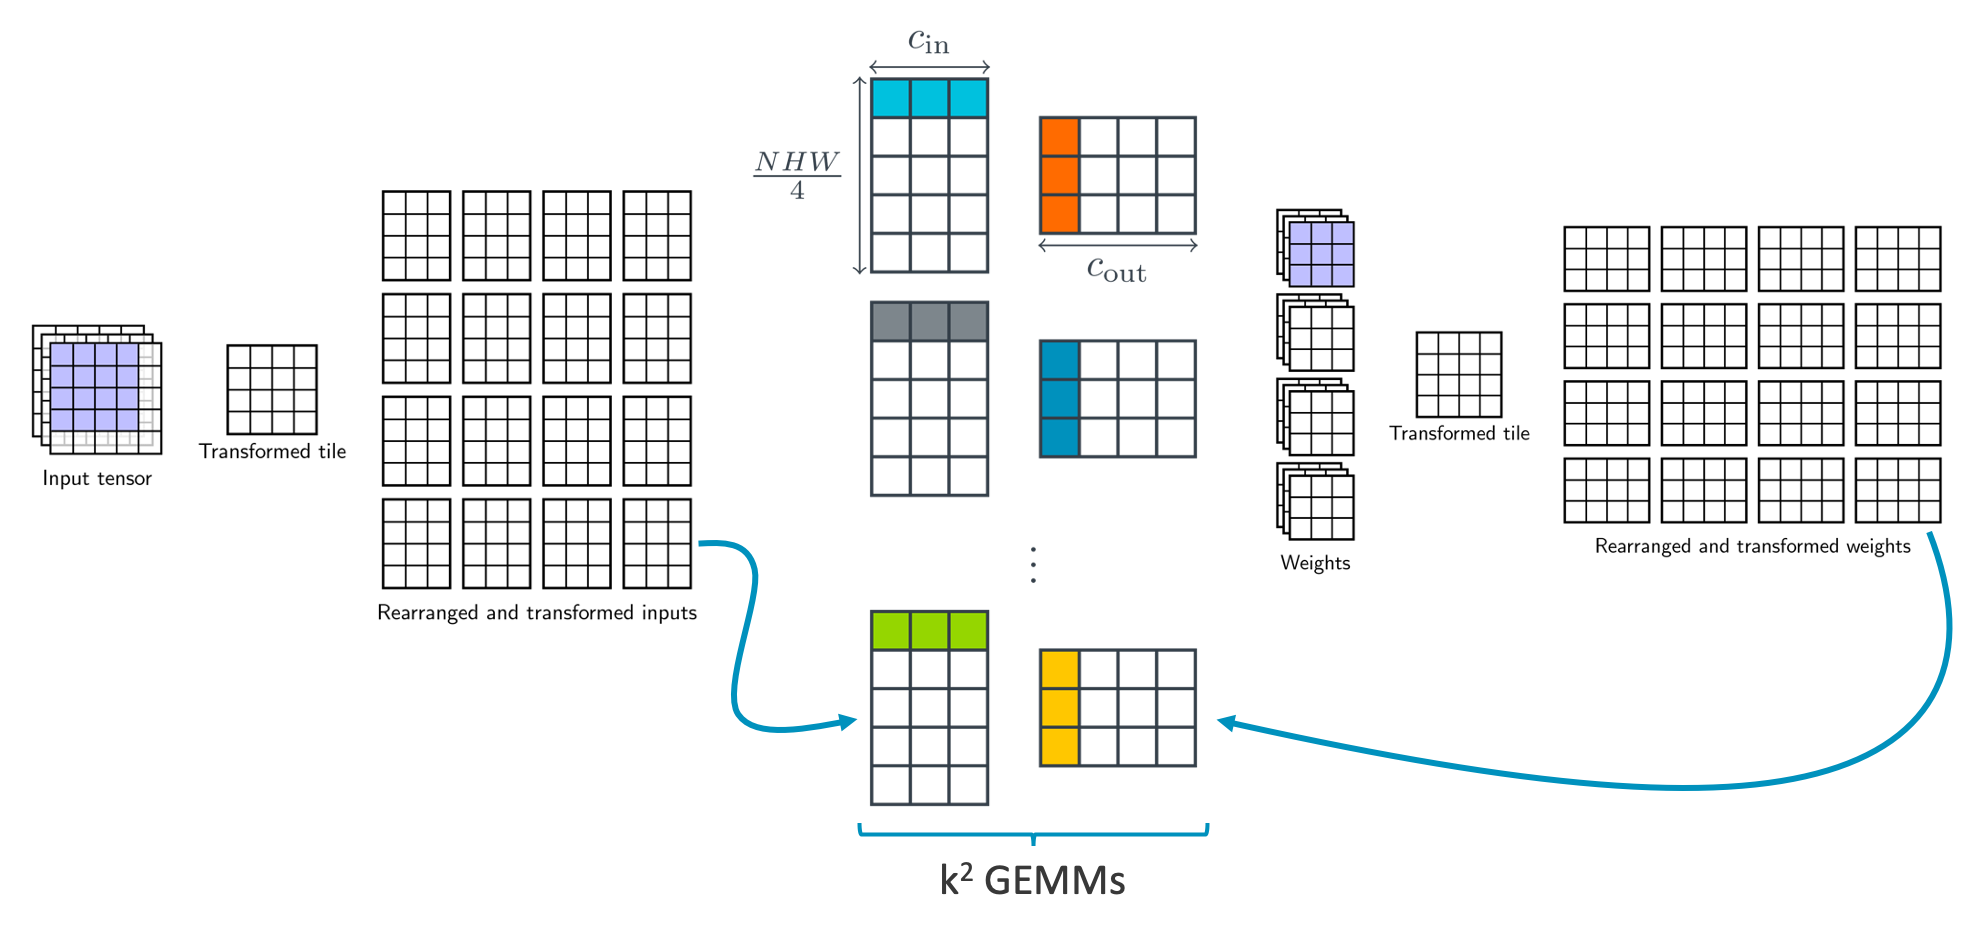
\includegraphics[width=\columnwidth]{winograd_conv_process}
\caption{ARM 设备Winograd卷积实现}
\label{fig:winograd_full_procedure}
\end{figure}

\section{高效量化矩阵乘法实现}

在输入和权重均经过Winograd 变换之后,变换后的矩阵会执行元素间的乘法,然后将对应位置的乘积结果累加(element-wise addition of Hadamard products)。
表示输出通道为m,输入通道为c的权重值可以在c通道中的所有输入区域被复用,
而 c 通道中位置为 $(i, j)$ 的输入则在所有的$(i,j )$位置输出的区域被复用。 这一观察表明,实际上这一操作本身可以转化为研究较为充分的通用矩阵乘法(GEMM)。
对于输入的channel数为 C,输出的channel数为M,且具有R 个分块的卷积, 在 $F(2, 3)$ 的Winograd 卷积中输入的元素为16个,那么对应的需要执行16 次 $[RxC]x[CxM] $
的矩阵乘法。

ARM 设备上没有成熟通用的矩阵乘法实现,特别是针对于量化场景的矩阵乘法计算。另外一方面,高性能计算(HPC)领域实现的矩阵乘法,并不同移动设备上的卷积网络的运算完全相匹配。HPC领域所设计的矩阵乘法面向的是上千维度的浮点数矩阵乘法,而本文所面对的,是矩阵维度从数十到数百近千不等的16位整数乘法。HPC领域的典型的优化矩阵乘法仍然有着相当的参考意义,然而在优化矩阵乘法过程中的每一步操作都有着额外的开销,因此这里需要选择性的针对移动端卷积网络参数的特性设计优化的矩阵乘法实现。

高效的矩阵乘法实现需要考虑以下几点:

\begin{itemize}

  \item 参与计算的数值表示。不同类型的参数存储需求不同,实现同样的操作也需要使用针对各个数据类型的不同指令。另外,矢量寄存器是定长的,比如128位长的矢量寄存器只能同时处理4个32位值或者是8个16位值,因此数值表示也决定了并行算法设计。
  \item 矩阵的规模。在矩阵的规模较小时,最为朴素的矩阵乘法实现并没有表现出性能问题,而当矩阵规模变大时,尽管问题的复杂度没有变,但是朴素的矩阵乘法并不能充分利用处理器的并行能力和存储的层次化结构,从而计算性能大幅下降。而各类优化矩阵乘法的方法,其适用性均是在一定的运算规模下的,盲目使用优化方法可能导致性能提升有限,反而引入了额外的开销。
  \item 并行加载/存储支持。数据的计算和加载在处理器中是由不同的单元实现的,而数据也只有在被加载到积存器中之后才能被用于计算。寄存器之间的操作远远快于寄存器同内存之间的操作,为提高计算性能,需要最大化计算/访存比,单次访存操作实现多个参数的加载和存储的能力,对此有着重要的意义,而在算法的调度上也必须满足,单次加载的多个数据被充分利用之后,再被并行存储。
  \item 矢量寄存器的位数及数量。这一点相当程度上代表了处理器的并行能力。更长的矢量寄存器意味着单个SIMD指令可以同时实现更多数据的计算,而矢量寄存器的数量又决定了可以有多少这样的并行计算可以同时执行。
  \item 乘累加指令操作延时(latency)。单个乘累加指令需要多个时钟周期完成,指令延时的存在需要结合pipeline考虑对于算法效率的影响。单个乘累加指令会存在较高的延时,而乘累加操作确实矩阵乘法中最为频繁使用的指令,而pipeline可以减小指令的平均延时,提高计算效率。算法的调度中要减少数据依赖,从而避免pipeline stall。
  \item 缓存信息,包括缓存行(cache line)大小,缓存放置策略(cache placement policy),缓存置换策略(cache replacement policy)。缓存的置换策略一般考虑LRU。缓存行的大小影响到线程并行化中数据分配的设计,要使得多个线程的数据不要处于同一缓存行,造成 Cache False Sharing,大幅拉低效率。同时缓存大小需要结合数据规模和计算执行的模式考虑,在一般的ARM Cortex A 芯片的多级缓存中,会具备两级缓存,L1 缓存速度远远高于L2缓存,但L1 缓存的容量远小于L2缓存,同时L1 缓存分为数据缓存和指令缓存。因此算法设计中,需要将频繁使用的数据放在L1 缓存中,而且这一部分数据要足够小,从而可以为L1 缓存所容纳,而复用程度相对较低的数据可以放在L2 缓存中。同时,算法中最为密集的计算,模型不能够不复杂,否则会造成指令缓存的浪费,引起性能下降。

\end{itemize}

以下将针对于ARM Cortex A架构的特征和轻量级量化网络中的参数特征,考虑上述高效矩阵乘法计算的要点展开阐述。在正式介绍矩阵乘法的算法设计之前,由于Winograd算法和矩阵乘法中都存在着频繁的对于多维矩阵的索引(indexing)及交换(permutation)操作,在\ref{sec:matrix_repr} 章节中先对于本文所采取的内存结构中多维矩阵的表示做简要介绍,这一矩阵表示方式可以实现简单且高效的索引机制,同时尽可能规避开销较大的交换操作。\ref{sec:hwchar} 章节中则对于ARM Cortex A架构硬件的特性做概述,作为\ref{sec:matrix-mul} 章节中的矩阵乘法设计作为背景。


\subsection{矩阵在内存中的灵活表示}
\label{sec:matrix_repr}
矩阵在存储空间中是以一整块连续的存储块空间所表示的。在矩阵的存储(storage)中有两个同内存(memory)相关的的关键问题:维度(dimension)和跨度(stride)。

跨度是指在遍历矩阵的过程中,在通过不同维度的过程中需要跨过的字节(bytes)数。跨度的存在可以使得很多矩阵的处理变得更加快速有效,同时,对于跨度的理解也有助于
更加容易的理解矩阵操作的实现。矩阵存储在被成为data buffer 的连续(contiguous)的同质(homogeneous)内存块( block of memory)中。Strides 可以作为一个
矩阵的meta data(元数据)实现多维矩阵之中的不同维度的index(索引)与它在连续memory block中的位置的映射(mapping)。简而言之,strides表示对于每个维度
的连续元素之间的字节间距(byte-separation)。同时矩阵存储空间的同质性也保证了矩阵在存储空间中的连续元素间的单位距离的一致性,比如对于int32类型的矩阵,
这里计量矩阵元素的单位距离就是 4个bytes,每两个矩阵元素在存储中的距离为4。于是对于多维矩阵而言,比如对于int类型的二维矩阵 $A$,$A$ 在矩阵表示的最内侧
的元素在memory中连续存储 ,即二维矩阵中的column(列)元素在实际的存储中相邻,在二维场景下可以成为 row-major。从$A[0, 0]$所表示的元素
移动到$A[0,1]$所表示的元素,即在同一行(第0行)中的元素间,从第0列移动到第1列,这里需要在data buffer中移动4个byte,也就是在列所对应的维度上的一个stride。
然而,如果从$A[0,0]$ 所表示的元素的位置移动到 $A[1, 0]$, 即在同一列(第0列),移动到下一行(从第0行移动到第1行)所在元素的位置,直观而言,需要先遍历
这一行中剩余的元素,才能够到达下一行,然后再下一行中遍历元素到达目标元素,比如矩阵$A$是一个$3x3$大小的矩阵,那么从 $A[0,0]$ 到$A[0,1]$ 需要遍历
$3x4$ 个bytes。也就是说矩阵$A$在行的维度上相邻元素间的间距(row stride)是 12个 bytes。Stride 的存在可以使得矩阵的处理变得更加灵活,也使得很多矩阵操作轻量化,矩阵的转置
以及reshape等操作可以不用实际操作矩阵,而仅仅是改变矩阵各个dimension 所对应的stride这一meta data,比如矩阵的转置实际上可以只是交换对应的stride并且
改变矩阵的shape信息。比如,对于前面例子中的3x3矩阵$A$,假如这里使用$(12, 4)$表示矩阵 $A$在第0维度(row)的stride为 12 个bytes,而在第1维度(column)
的stride为 4个bytes。它的转置$A^T$并不需要对于$A$所对应的内存块中的元素做实际的重新排布 (reorder),而只需要将 $A$原本所对应的stride信息修改为
$(4, 12)$ 即可。同样的,在考虑到矩阵的stride这一元信息(meta info)的场景下,对于举证的处理也不能直观的认为矩阵的最内层(innermost)元素之间的距离
一定是单位该元素数据类型的尺度。而是在沿着矩阵的某个维度实现遍历处理的过程中,这一维度上对应元素间的距离一定是这一维度队对应的stride。

除其他外,基于原有的矩阵的创建一个新的矩阵对象的操作也可以因此而轻量化。创建一个新的数组元数据,该元数据使用相同的data
buffer 来创建该数据缓冲区的新视图,该视图对缓冲区的解释(interpolation)不同(例如,形状,偏移量,字节顺序, 大步等),但共享相同的数据字节。 例如slice 操作,
只需要创建一个新的矩阵元数据信息,对应的更改其起始位置的offset和各个维度的stride,而不需要从memory中拷贝data buffer中的相关数据元素。

\subsection{ARMv8-A 架构硬件特征}
\label{sec:hwchar}

ARMv8 指令集架构的设计中包含 32个64位 (doubleword)NEON 寄存器,或者称为 D 寄存器,同时,这32个 D 寄存器也可以视为 16 个 128位(quadword)寄存器,
称为 Q 寄存器。

NEON 作为一个SIMD 并行计算的协处理单元,具有以下流水线执行特征
\begin{itemize}
\item NEON指令运行在其独立的10-stage 的流水线中
\item ARM 在每个执行周期(cycle)可以调度(dispatch)两个NEON 指令
\item 可以容纳16条指令的指令队列(16-entry instruction queue)可以用于在指令实际进入pipeline之前作为缓冲
\item 可以容纳12条数据记录的队列用于存储ARM 寄存器的值,在ARM调度指令之后保存当时ARM 寄存器的值
\end{itemize}

由于以上的特征,在实现ARMv8 指令集的大多架构下,由ARM到NEON(由CPU 处理器到 SIMD 协处理器)的数据传输是相对高效迅速的,而由NEON到ARM 的数据传输则相对
有较高的延时(latency);
同时在ARM 处理器一方不会因为 NEON 协处理器的执行而停滞,除非NEON 协处理器的队列已满。ARM 处理器可以向 NEON 协处理器调度分布一系列的指令后继续处理器
本身的任务,直到NEON 指令的结果返回;
另外,NEON 指令的实际执行同在编写代码中直观观察到的执行并不是一致的,由于队列的存在,NEON 指令的实际执行是有所延后的。这就导致,如果由程序修改了另外一个
程序所需要的缓存行(cache line),会导致ARM 处理器侧的停滞,直到NEON的执行同步。

\subsection{硬件相关的矩阵乘法性能优化}
\label{sec:matrix-mul}

根据前文对于矩阵乘法实现要点的分析,以下将针对于各个要点展开。具体而言,体现为如下具体步骤:

\begin{itemize}
  \item 首先确定问题建模。确定矩阵乘法计算中的数据类型以及矩阵乘法的规模;
  \item 硬件层级自底向上分析各个层级的最高效实现,包括: 
    \begin{itemize}
      \item 指令层级:并行访存指令和并行计算指令下的基本算法单元;
      \item 寄存器层级:最小化加载/存储操作,提升计算/访存比;
      \item 缓存层级:充分利用缓存性能,尽可能减少访存开销;
   \end{itemize}
\end{itemize}

\subsubsection{量化计算中的数据表示}

讨论数字格式(numerical format)时,有两个主要属性。第一个是动态范围,它是可表示数字的范围。
第二个是动态范围内可以表示多少个值,这又决定了格式的精度/分辨率(两个数字之间的距离)。

对于所有整数格式,动态范围为[-2n-1..2n-1-1],其中n是位数。因此,对于INT8,范围是[−128..127],
对于INT4,范围是[−8..7]。整数型数字可表示值的数量为$2^n$。而32位浮点数的动态范围为$\pm3.4 x 10^38$,
可以表示大约$4.2 x 10^9$的值。 这里可以立即发现FP32更具通用性,因为它能够准确地表示各种分布。
这的确是满足深度学习模型需求的一个属性,在深度学习模型中,权重和激活的分布通常非常不同
(至少在动态范围内)。此外,模型中各层之间的动态范围可能会有所不同。 为了能够用整数格式
表示这些不同的分布,比例因子(scale factor)可以被用于将张量的动态范围映射到整数格式范围
。但是,相比于浮点数,整数可表示值的数量要少得多,即分辨率要低得多。
在很多情况下,比例因子可以是浮点数。因此,即使使用整数,也会保留一些浮点计算。另外一方面,
乘法运算也可以使用位移(shift)实现,这样可以不必乘以scalar factor,从而消除了浮点运算。
在GEMMLWOP中,原本未32位浮点数的比例因子便是使用整数乘法加上移位运算来近似得出的。
在许多情况下,这种近似对精度的影响可以忽略不计。

卷积和完全连接的层涉及将中间结果存储在累加器(accumulators)中。 由于整数格式的动态范围有限,
如果我们将相同的位宽用于权重和激活以及累加器,则可能会很快溢出。 因此,累加器通常以更高的位
宽实现。

两个n位整数相乘的结果最多为2n位数字。 在卷积层中,此类乘法被累加$c·k^2$次,其中c是输入通道的
数量,k是内核宽度(假定为正方形内核)。 因此,为避免溢出,累加器应为$2n + M$位宽,其中M至少
为$\log_2(c⋅k^2)$。 在许多情况下,使用32位累加器,但是对于四位整数及更低版本,可能会使用少于
32位的累加器,具体取决于预期的使用情况和层宽度。

因此,可以确定在Winograd 卷积中使用的累加器为32位整数,即这里矩阵乘法的结果将保存为32位整数。
而另外一方面,量化场景下卷积网络中的参数和特征的表示均为8位无符号整数,而在实现Winograd变换中
为了尽可能保持数值精度,变换过程中将输入转换为16位有符号整数计算,并将变换后的结果以16位整数
存储。到此为止,可以确认,参与矩阵乘法的输入的数据类型为16位整数,输出为32位整数。

\subsubsection{轻量化网络中的矩阵乘法规模}

不同的网络中参数的规模会存在比较大的差异,在网络计算中实现的矩阵乘法的规模也随之会处于比较大的
变化范围。表\ref{tbl:conv-matmul} 中对比了VGG19 和 ResNet18 中的卷积操作的参数规模,以及各自对应到Winograd卷积中的
矩阵乘法的参数规模。由于本文实现的Winograd卷积只针对于 stride 为1的3x3卷积操作,因此表\ref{tbl:conv-matmul}中也只统计计算了网络中满足这一条件的卷积,但其中所统计的卷积已经占据了网络结构中的绝大多数卷积操作,对于这些卷积操作的统计结果在很大程度上也反映了整个网络运行时的性能。

\begin{table}[]
  \centering
  \caption{卷积网络中的卷积操作参数以及在Winograd卷积中对应的矩阵乘法。卷积核参数后的括号内表示该卷积操作在网络中的重复次数。}
  \begin{tabular}{cccc}
    \toprule
    网络 & 输入(HxWxC) & 卷积核 (CxHxWxK) & 矩阵乘法(AxB) \\
    \midrule
    \multirow{9}{*}{VGG19} & 224x224x64 & 3x3x3x64 & (12544x3)x(3x64)\\
                          & 224x224x64 & 64x3x3x64 & (12544x64)x(64x64)\\
                          & 112x112x64 &  64x3x3x128 & (3136x64)x(64x128)\\
                          & 112x112x128 &  128x3x3x128 & (3136x128)x(128x128)\\
                          & 56x56x128 & 128x3x3x256 & (784x128)x(128x256)\\
                          & 56x56x256 & 256x3x3x256 (x3) & (784x256)x(256x256)\\
                          & 28x28x256 & 256x3x3x512 & (196x256)x(256x512)\\
                          & 28x28x512 & 512x3x3x512 (x3) & (196x512)x(512x512)\\
                          & 14x14x512 & 512x3x3x512 (x4) & (49x512)x(512x512)\\
    \hline
    \multirow{4}{*}{ResNet18} & 56x56x64 & 64x3x3x64 (x4) & (784x64)x(64x64)\\
                             & 28x28x128 & 128x3x3x128 (x3) & (196x128)x(128x128)\\
                             & 14x14x256 & 256x3x3x256 (x3) & (49x256)x(256x256)\\
                             & 7x7x512 & 512x3x3x512 (x3) & (16x512)x(512x512)\\
    \bottomrule
  \end{tabular}
  \label{tbl:conv-matmul}
\end{table}

显然,轻量级的卷积网络在矩阵乘法中所处理的问题规模同传统的卷积网络相比是截然不同的。轻量化的网络中需要解决的
矩阵乘法问题的规模远小于传统的卷积网络。此外,在本文所针对的量化计算场景下,数据在存储设备(内存,缓存,寄存器)中的开销将变得更小。


至此,已经完善了对于应用于移动端的量化Winograd卷积中,矩阵乘法问题的建模。总结而言,这里需要解决
的问题是,中小规模的16位整数矩阵的乘法,乘积则为32位整数表示。 为方便后文表述,这里定义两个矩阵 $A$, $B$, 对应的尺度分别位 $m x k$, $k x n$, 记为 $A(m, k) $ 和 $ B(k, n) $, 则两者的矩阵乘积可以表示为

\begin{align}
  C(m, n) = A(m, k) x B(k, n)
\end{align}

直观而言,矩阵乘法可以视作是矩阵A 中的行同矩阵 B 中的对应的列的点积的集合,是对应矩阵元素的乘积的和(sum of element-wise multiplication)。简单的伪码
实现如下:

\begin{lstlisting}[label={code:matmul_naive}, caption={矩阵乘法}]
  for (int i = 0; i < m; i++) {
    for (int j = 0; j < n; j++) {
      for (int p = 0; p < k; p++) {
        C(i, j) += A(i, p) * B(p, j);
      }
    }
  }
\end{lstlisting}

对这一简单直接的矩阵乘法的实现的可视化可如下图\ref{fig:naive_matmul}所示

\begin{figure}
\centering
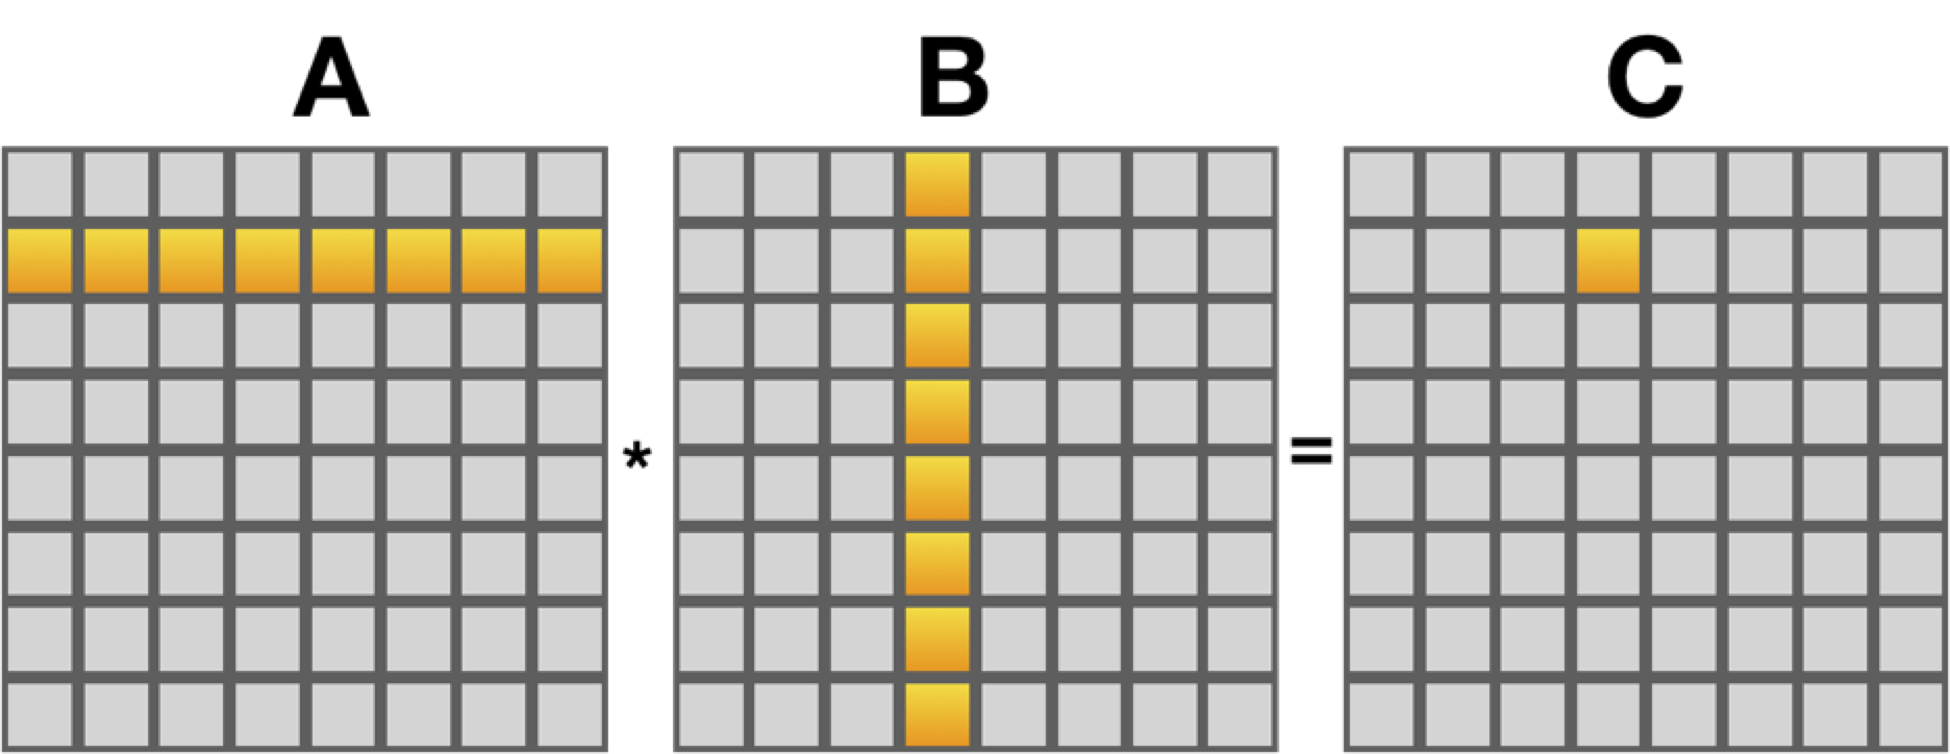
\includegraphics[width=0.8\columnwidth]{matmul_naive.png}
\caption{naive 矩阵乘法}
\label{fig:naive_matmul}
\end{figure}

而一个针对于高性能计算场景下的矩阵乘法计算则需要针对性的实现多层级的优化。以BLIS\cite{BLIS1}为例,其中的矩阵乘法的
实现策略如图\ref{fig:blis-gemm} 所示。

\begin{figure}
  \centering
  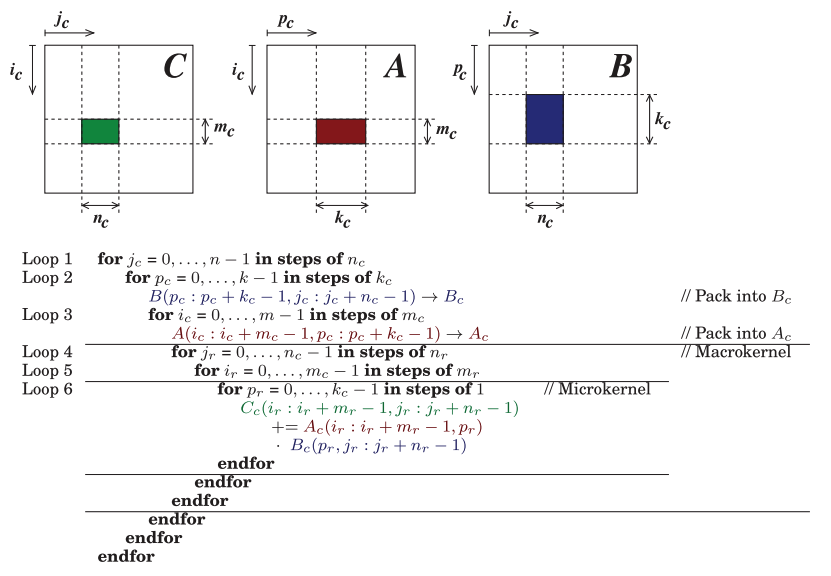
\includegraphics[width=0.8\columnwidth]{high-perf-gemm}
  \caption{矩阵乘法的高效实现。图片来自BLIS\protect\cite{Low2016AnalyticalMI}}
  \label{fig:blis-gemm}
\end{figure}

而对于上述矩阵乘法计算的图形化表示可以参见图\ref{fig:gemm} 。总体来看,图\ref{fig:gemm} 中自上而下,同图\ref{fig:blis-gemm} 中所描述的算法循环从外而内相对应,而对于矩阵乘法而言,也意味着问题的分析由宏观入微观。在对于矩阵乘法问题分解的角度而言,这里由外而内针对的问题对象分别是矩阵,缓存块(cache block),寄存器块(register block),寄存器内的矢量(vector)。从计算实现的角度而言,由外及里则分别是矩阵乘法(GEMM),Macro Kernel和 Micro Kernel。从问题处理的规模而言,则由外而内依次减小。换言之,工作\cite{BLIS1} 中的优化策略将矩阵乘法自上而下分解为一系列规模递减的问题,在不同规模的层次上有着针对性的优化方法。正因如此,结合前文中对于本文所涉及的矩阵乘法问题的分析,以下便可以结合本文问题的规模,针对性的实现中小规模量化矩阵的高效乘法实现。

\begin{figure}
\centering
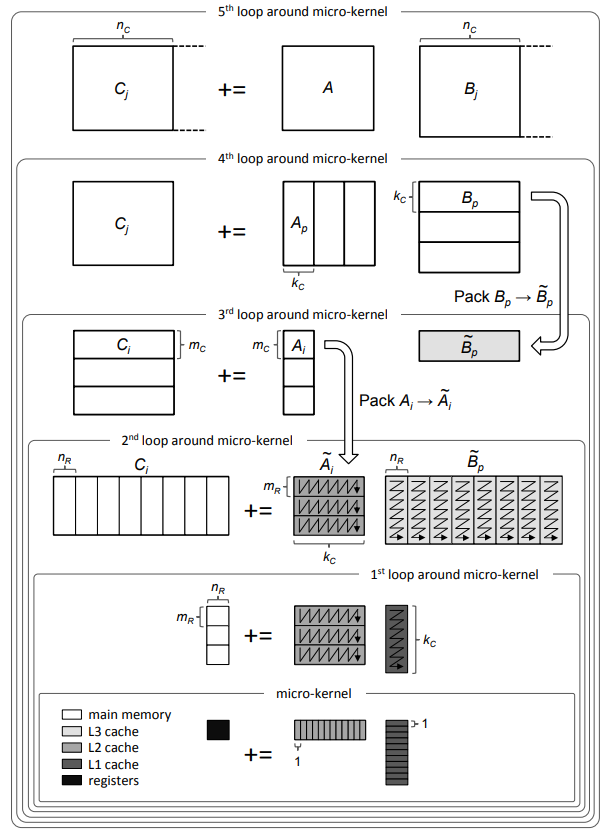
\includegraphics[width=\columnwidth]{gemm.png}
\caption{高效GEMM实现。图片来自BLIS\protect\cite{Low2016AnalyticalMI}}
\label{fig:gemm}
\end{figure}

在此之前,仍然有必要简要介绍\cite{BLIS1} 中的矩阵乘法实现。对于矩阵乘法问题自上而下的分解,实际上是同具体的硬件特征相关的。图\ref{fig:gemm-hw} 大致上描述了这一算法中各级子问题同硬件设备的对应关系,同时也是算法实现中各个层级之间数据在不同硬件设备上转移的流程。首先,关于自上而下的子问题的拆分,
在如图\ref{fig:gemm}所示的矩阵乘法算法中。在最高层次上,将大小为m,n和k的矩阵乘法在 k 所表示的维度以$k_c$ 大小的高速缓存块进行分割,从而创建rank为k的子问题。 在这一阶段,
为了实现在计算的最基础层次上上,参与计算的元素在存储中是完全连续的,即矩阵表示中最低维度对应的stride为unit stride,需要将B以一种特殊的格式分块打包到连续存储中
(标记为B )。 然后,将每个rank为k的子问题沿m维度,按照缓存块大小$m_c$分块,从而创建block-panel子问题。 然后将当前的$m_c×k_c$块, 记为$A_i$, 按照计算中的
最基础级别,参与计算的元素在存储中是连续的的原则,打包到A。 然后将剩下的该block-panel子问题($C_i = C_i + A_i B$)实现为高度优化的汇编
计算内核。 而该内核将继续沿$n$,$m_c$划分矩阵,最后在$k_c$维划分矩阵。
另外,从数据的转移角度来说,即考虑存储设备的访问开销,这种对于问题的划分也是基于频繁复用的数据应该尽可能存储在高速存储设备中的原则。

\begin{figure}
  \centering
  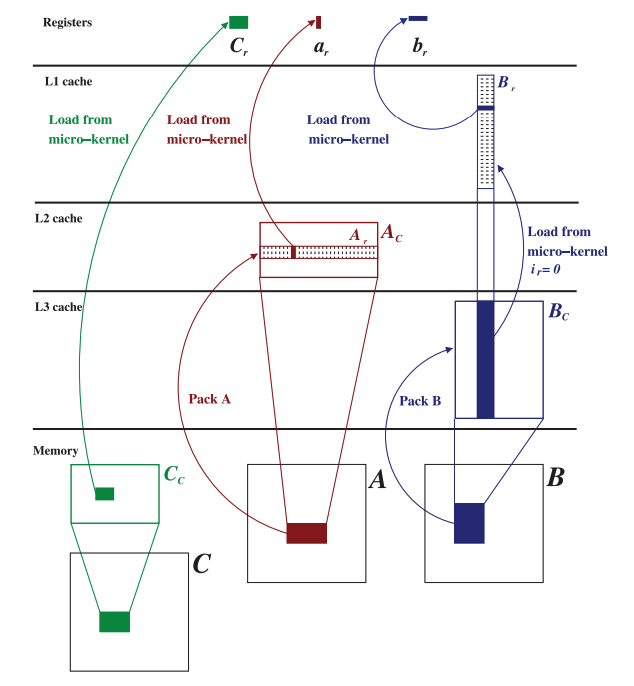
\includegraphics[width=0.8\columnwidth]{data-mov-gemm}
  \caption{矩阵乘法子问题与硬件关联。图片来自\protect\cite{Low2016AnalyticalMI}}
  \label{fig:gemm-hw}
\end{figure}

这一矩阵乘法中的多个循环的使用在于根据缓存块大小和寄存器的容量,精心设计矩阵的分块策略,从而使得子矩阵的分布同存储的层级结构相匹配,以达到数据复用的目的。
同时A 和B 的子矩阵被复制打包到临时工作区(workspace),从而使得矩阵乘法操作的micro-kernel能够在内存中连续访问矩阵元素,从而提高了缓存和TLB性能。而一般
打包过程的成本可以通过计算本身来摊销,在计算的规模足够大时,这一成本是可以忽略不记的。

而这其中决定最内层的循环的调用的寄存器相关的参数 $m_r$, $n_r$, 以及较外层的循环调用的高速缓存相关参数 $m_c$, $k_c$, $n_c$ 一般由具体硬件的特性所决定,
比如矢量寄存器的大小,缓存大小,缓存的相关性等。\cite{Low2016AnalyticalMI}为这些参数的选择提供了一种分析性模型。


至此,对于本文解决的Winograd卷积中的矩阵乘法的分析,以及一般意义上的高效矩阵乘法的实现阐述均已完备。以下将自下而上,从问题实际和硬件特性的角度针对性的设计矩阵乘法。

\subsubsection{SIMD矢量化矩阵乘法计算基本单元}
\label{sec:linear-matmul}

首先针对于矩阵乘法计算中的最内层,在矢量级别处理矩阵乘法的计算。考虑硬件提供的并行数据加载机制,在ARM Cortex A设备上,可以单次加载多个顺序存储的数据到NEON 矢量寄存器中。这意味着,在加载矩阵中的元素时,针对于16位整数,一个加载指令可以最多加载8个同一行中的矩阵元素。考虑矩阵乘法 $A \times B = C$ ,$ C$ 中第$ i$ 行,第$j$ 列的值,有 $A$ 中第 $i$ 行的所有元素,同第$j$ 列的所有元素的点积确定。而这里的并行加载机制对于访问矩阵中的列元素的支持是不友好的。比较直接的一种方案是对于B中的元素做转置,转置之后,B 矩阵中的元素便也可以发挥并行加载指令的优势,减少存储访问。但转置本身是一个成本比较高的操作,因此这里考虑另外一种优化策略,从矩阵乘法的计算方式角度,提出解决方案。

矩阵乘法有一个属性在于:矩阵 A 乘 矩阵 B 实际上是将矩阵A 中的列以矩阵 B 中的列元素作为参数的线性组合,或者说是,矩阵 B 中的行已矩阵 A 中的行元素作为参数的线性组合。

首先,矩阵的右乘,可以视作列的组合;对于简单的矩阵右乘一个列向量的情形

\begin{equation}
  \begin{pmatrix}
    x_1 & y_1 & z_1\\
    x_2 & y_2 & z_2\\  
    x_3 & y_3 & z_3
  \end{pmatrix}
  \times 
  \begin{pmatrix}
    a \\
    b \\
    c
  \end{pmatrix}
  = 
  \begin{pmatrix}
    ax_1 + by_1 + cz_1\\
    ax_2 + by_2 + cz_2\\  
    ax_3 + by_3 + cz_3
  \end{pmatrix}
\end{equation}

而对于这一过程做一个直观的可视化可以表示为图\ref{fig:matvec}

\begin{figure}
\centering
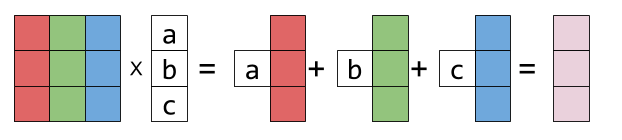
\includegraphics[width=0.8\columnwidth]{matvec.png}
\caption{列向量右乘矩阵}
\label{fig:matvec}
\end{figure}

矩阵中的每一列同列向量中的每个元素相乘,矩阵中的一列同列向量中的单个元素(Scalar)的乘积仍是一个列向量,而最终的结果则是这些列向量的和。
这一情形推广到右乘一个矩阵则是相似的情形,乘积的结果的矩阵中的每一列仍是矩阵列的线性组合。

\begin{equation}
  \begin{pmatrix}
    x_1 & y_1 & z_1\\
    x_2 & y_2 & z_2\\  
    x_3 & y_3 & z_3
  \end{pmatrix}
  \times 
  \begin{pmatrix}
    a & d & g\\
    b & e & h\\
    c & f & i
  \end{pmatrix}
  = 
  \begin{pmatrix}
    ax_1 + by_1 + cz_1 & dx_1 + ey_1 + fz_1 & gx_1 + hy_1 + iz_1 \\
    ax_2 + by_2 + cz_2 & dx_2 + ey_2 + fz_2 & gx_2 + hy_2 + iz_2 \\
    ax_3 + by_3 + cz_3 & dx_3 + ey_3 + fz_3 & gx_3 + hy_3 + iz_3
  \end{pmatrix}
\end{equation}

这一过程的可视化表示如图所示为图\ref{fig:matmul_right}

\begin{figure}
\centering
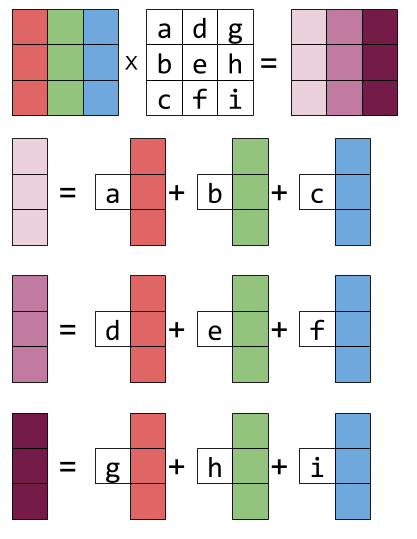
\includegraphics[width=0.6\columnwidth]{matmul_right.png}
\caption{矩阵右乘}
\label{fig:matmul_right}
\end{figure}

而对于左乘一个矩阵则可以视为是矩阵行的线性组合。首先对于一个矩阵左乘一个行向量的情形,可以表示为

\begin{equation}
  \begin{pmatrix}
    a & b & c
  \end{pmatrix}
  \times
  \begin{pmatrix}
    x_1 & y_1 & z_1 \\
    x_2 & y_2 & z_2 \\
    x_3 & y_3 & z_3 
  \end{pmatrix}
  = 
  \begin{pmatrix}
    ax_1 + bx_2 + cx_3 & ay_1 + by_2 + cy_3 & az_1 + bz_2 + cz_3
  \end{pmatrix}
\end{equation}
可视化表示为\ref{fig:vecmat}

\begin{figure}
\centering
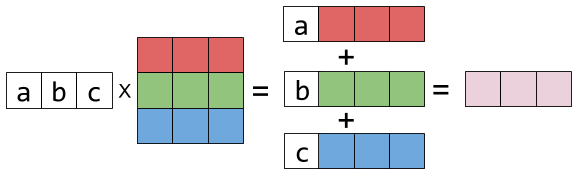
\includegraphics[width=0.8\columnwidth]{vecmat.png}
\caption{行向量左乘矩阵}
\label{fig:vecmat}
\end{figure}

而在左乘一个矩阵的过程中,则是左乘行向量的情形重复作用于矩阵中的每一行。相对应的可视化表示可以为图\ref{fig:matmul_left}

\begin{figure}
\centering
  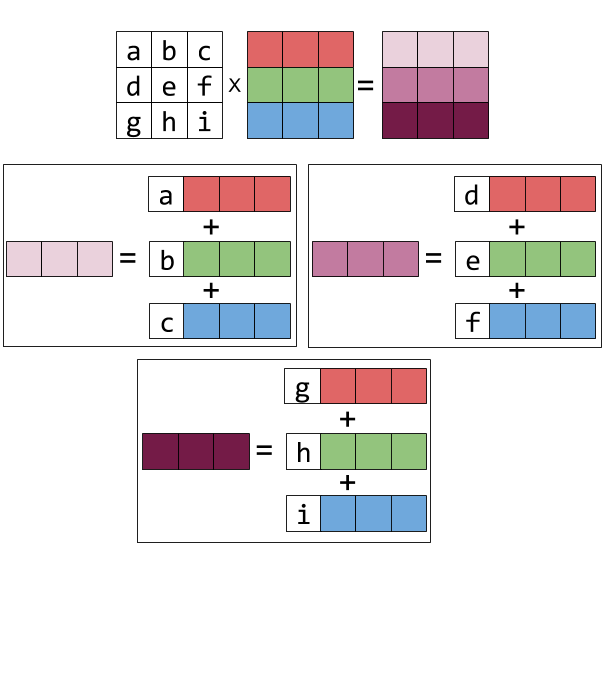
\includegraphics[width=0.6\columnwidth]{matmul_left.png}
\caption{左乘矩阵}
\label{fig:matmul_left}
\end{figure}

而另外一方面,ARM Cortex A架构的NEON指令中是支持 按照矢量寄存器的 data lane 进行计算的,因此可以
加载 矩阵A 同一行中的多个元素到矢量寄存器 R,
再将R中各个data lane的元素分别同B中同一行的多个顺序元素分别相乘。对于B中的多行元素重复上述步骤,
便得到矢量同矩阵的乘积结果。再对于A中的多行元素重复矢量-矩阵乘法,并对结果实现前述的线性组合,便得到
矩阵乘法结构。

至此,本文针对于硬件的数据加载结构和计算指令的data lane特征,利用矩阵计算的线性组合性,对于矩阵乘法
的基本实现单元实现了修改。下文中将在较高的层次,矢量寄存器级别,实现对于矩阵乘法的优化。

\subsubsection{矢量寄存器分块化处理-- 优化最内层循环}
\label{sec:register-block}

众所周知,寄存器对于数据的操作,总体上存在三个阶段:加载,计算和存储写出。对于计算的执行而言, 
现代CPU 一般存在
多个用于调度分配SIMD 计算的执行端口,和多个用于调度数据存取的端口。这意味着,在一个时钟周期里可以实现调度执行多条读取数据的指令,或者
调度执行多条乘法计算指令。而在存储访问方面(数据加载和写出),从读写的速度考虑,处理器中的寄存器间的操作的速度是远远高于缓存的读写性能,而缓存的读写性能又远远高于内存,内存的
读写性能则又远远高于硬盘等外部存储。计算机存储结构的设计是层次化的,算法设计中对于存储设备的访问也需要遵守这一特性。高效计算的过程中对于存储性能的优化的目标在于,尽可能的减小访问存储的操作同计算操作的比例,提高
高速设备中数据的利用率,在算法的设计上保证加载到高速设备上的数据得到充分利用,并可复用。而在实现矩阵乘法的背景下,这就意味着,从矩阵 A 中
加载的数据需要被用来执行多次计算操作,这一点可以由\ref{sec:linear-matmul}章节所述方法中,A 中的元素同来自B 中的同一行中不同列的元素做计算而保证;同时,
B 中的元素也需要被用于执行不止一次计算,而要实现这一点,则可以通过加载数据时,从矩阵 A 中每次加载多行的元素,从而使得B 中的每一列的元素
可以得到复用。而从计算结果来看,乘积矩阵 C 中的每一行的元素都是一个矢量累加值,并且对应于矩阵A中的行,每次处理多行A 中的元素,需要在计算中具备与之数目相同的累加器用来暂时存储矩阵 C 的结果。这一过程中使用了多个寄存器实现了矩阵中的一个小块(block)的计算,这一过程被称为寄存器 blocking (register blocking) 。

\begin{figure}
\centering
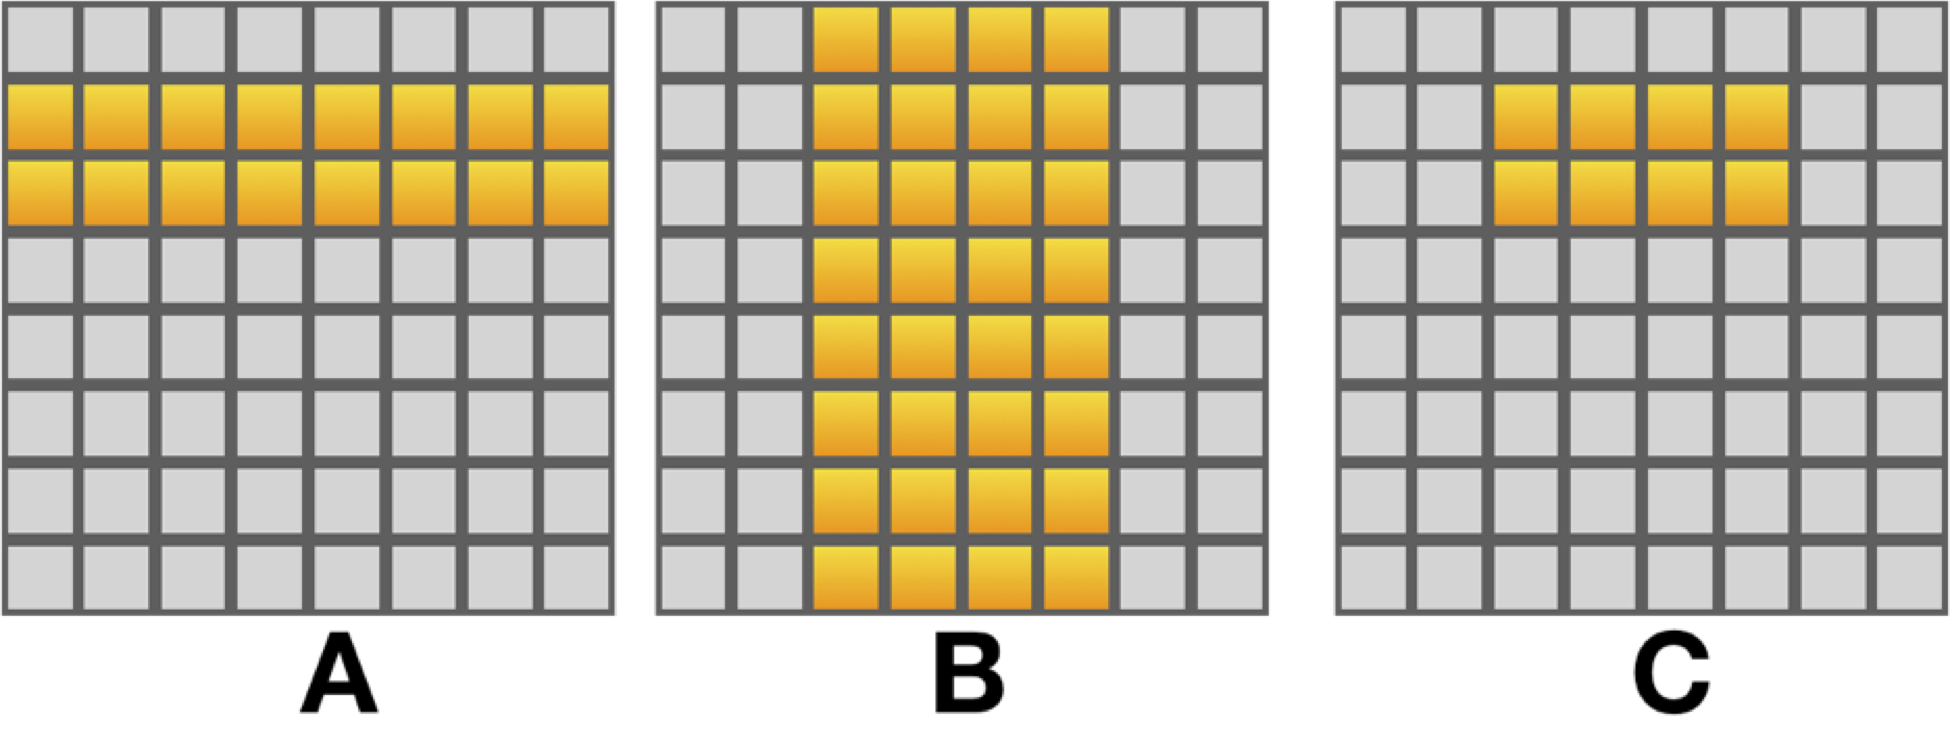
\includegraphics[width=0.8\columnwidth]{zregblock.png}
\caption{矩阵乘法实现 + Register Blocking}
\label{fig:zregblock}
\end{figure}

图\ref{fig:zregblock} 对于register blocking 实现做了比较直观的可视化。
一般register blocking 方法存在这两个参数,垂直方向的blocking size $m_r$ 和水平方法的blocking size $ n_r $。
这两个值的上限收到矢量寄存器的数目所限制,而当 $m_r$ 和$n_r$ 均为1 时,算法退化为朴素矩阵乘法。为了尽可能
避免数据依赖和指令操作延时导致的pipeline stall,$m_r$ 和$n_r$ 的取值应该足够大,但并不是越大越好。因为还需要
分配一部分寄存器作为累加器暂存结果矩阵C中的值。在单个的register blocking计算过程中,计算输出的
结果的维度为 $m_r \times n_r$, 因此用于暂存结果累加器的数目由$m_r$, $n_r$ 共同决定。寄存器总数有限,
这里要求用于暂存C中的输出的寄存器尽可能少,从而有足够多的寄存器用于计算矩阵A,B中的输入,因此这里的
blocking factor $m_r$, $n_r$ 的取值需要做一定的权衡。

工作\cite{Low2016AnalyticalMI} 中对于寄存器级别的blocking factor的选择提出了一种分析模型。从硬件参数
通过式\ref{eq:register-block-factor}可以推算合适的$m_r$ 和 $n_r$ 值。其中 $N_{VEC}$ 表示单个矢量寄存器
所能容纳的数据的数目,$N_{VFMA}$ 表示可执行矢量乘累加计算(Vector FMA)的寄存器的数目,而 $L_{VFMA}$ 则表示
乘累加计算的操作延时(latency)。

\begin{align}
  \label{eq:register-block-factor}
  m_r = \ceil[\bigg]{\frac{\sqrt{N_{VEC}L_{VFMA}N_{VFMA}}}{N_{VEC}}} N_{VEC} \\
  n_r = \ceil[\bigg]{\frac{N_{VEC}L_{VFMA}N_{VFMA}}{m_r}}
\end{align}

由这一过程推算出的寄存器分块因子(register blocking factor) $m_r$ 和 $n_r$ 在大多情形下同成熟的矩阵计算库中通过经验型调优方法获得的值吻合。本文经过对于主流的ARM Cortex A设备的相关硬件参数值做统计,并结合本文实现的矩阵乘法背景设置,分别取 $m_r$,$n_r$ 的值为 8, 8。

此外,图\ref{fig:blis-gemm} 中的最内层循环,即Loop 6 中在$k_c$ 维度的循环中的步长为1 ,而本文的矩阵乘法在\ref{sec:linear-matmul} 中所述的矩阵乘法实现在最基本单元的单元,就已经确定了矩阵 A 的多行元素和矩阵 B 中的多列元素的并行化计算,这一设计将同时影响到packing策略,将在后文展开阐述。本文的实现中,考虑矢量寄存器长度和数量的限制,同时兼顾编译器的循环优化中的loop unrolling和数据预取(data prefetching),本文中取在 $k_c$ 维度的循环步长为 4 。

至此,寄存器级别的计算优化基本完善。以下将从计算机存储设备中的层次化结构中,数据存取速度次于寄存器的高速缓存的硬件特征,分析在矩阵乘法中计算规模更高一级的问题的优化。

\subsubsection{缓存优化策略讨论Packing 与 Blocking}

处理器每次从主内存中(main memory )中加载数据的过程中,会同时将该数据所处的一个缓存行(cache line )加载到 L1 高速缓存中,而此后参与计算的数据如果同该数据处于同一缓存行,那么CPU 只需从L1 缓存中加载数据,而不必访问需要较大储存访问开销的内存。缓存友好的数据组织方式要求参与计算的数据依次顺序排列在储存中。为实现数据访问模式的缓存友好性,可以针对于章节\ref{sec:register-block} 中所描述的计算模式,对于参与计算的数据重新排布。这一过程一般成为packing。Packing可以使得参与计算的数据均位于连续的存储中,最大化缓存命中率,同时还可以数据在缓存行(cache line)边界和内存页(page)边界对齐,从而可以使用访问对齐数据的指令,从而加速加速;此外,Packing 还更有利于数据在对应的各级缓存中的预加载。

在\ref{fig:blis-gemm} 中所描述的寄存器级优化方法下,矩阵 A 中的数据需要重新排列为column-major的格式,即储存中连续的数据处于同一列中,而这一过程需要将矩阵 A 转置。转置操作的计算开销不容忽略,而另外一方面,关联到神经网络中的应用,A 对应于特征输入,而B 则代表模型的权重。在网络模型的执行过程中,A 的值是不定的,网络每次的输入值在实际应用中是不同的,对于A的优化不能得到复用。综合这两点考虑,packing对于输入的矩阵A 的处理,所带来的计算效率提升将相当有限。

而在\ref{sec:register-block} 中所描述的矩阵乘法实现下,对于矩阵A 而言,计算过程中会有多列元素参与,在没有packing 的实现下会具有比\ref{fig:blis-gemm} 中方法更高的缓存效率。另外一方面,参考\ref{tbl:conv-matmul} 中的轻量级网络的参数规模,在量化场景下,L2 缓存的容量便可以满足A 中的参数量(这一点将在后面展开),这在一定程度上保证了A中数据的缓存效率底线。考虑矩阵乘法中的另一输入,矩阵B 的值是固定的,从而对于B 所执行的各种优化处理,则可以在每次的执行中被复用。并且这些处理可以在预处理阶段完成,而不给网络模型的运行时带来开销。矩阵B 的packing 需要按\ref{sec:register-block} 中的算法,将多行中的同列的 长度$n_r$的向量首位相接,如图\ref{fig:weight-packing}所示,按照Z 字形遍历矩阵,完成矩阵的重新排布。 

\begin{figure}
  \centering
  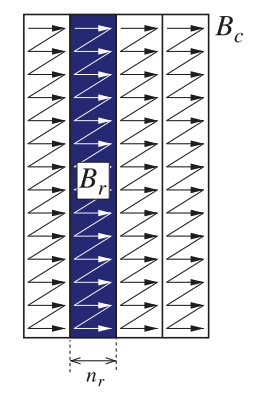
\includegraphics[width=0.4\columnwidth]{weight-packing}
  \caption{矩阵B 的packing策略}
  \label{fig:weight-pack}
\end{figure}

而在Intel 的CPU高性能计算库MKL 的实现中,有发现\ref{mkl_gemm_pack}表明尽管Packing 方法在较大规模的矩阵乘法中
有着比较明显的效率提升,但是在机器学习模型中常用的规模比较小的矩阵乘法中的性能提升效果有限,并且packing引入额外的开销无法在小规模
的计算中被充分摊销,从而甚至会引起性能的负向优化。本文将在后文中通过实验分析Packing 策略对于ARM Cortex A 设备
上的中小规模矩阵乘法效率的具体影响。

而在packing之外,另一可以有效提升缓存效率的方法为 Cache Blocking。Blocking 方法的目的在于减少对于内存带宽的压力,避开内存带宽瓶颈。Cache blocking 通过组织数据,将数据切分成适合缓存大小的块,将规模较大的矩阵中的一小部分加载到高速缓存中,并且在矩阵乘法实现中尽可能复用缓存中的矩阵子块,而不必访问存储开销更大的内存,提高缓存效率。

图\ref{fig:blis-gemm} 中的最外围的三层循环Loop1 ,Loop 2,Loop 3即是对于cache block的划分过程。而其内层的两重循环
Loop 4 和Loop 5 则代表了在Cache Block内部计算各个Register block 的过程。以下对于Cache Blocking 的实现做简要描述。

\begin{algorithm}
  \For{ $i \gets 1$ \KwTo N }{
    \For{ $j \gets 1$ \KwTo N}{
      read block $C_{i,j}$ to fast memory\\
      \For{ $k \gets 1$ \KwTo N}{
        read block $A_{i, k}$ to fast memory\\
        read block $B_{k, j}$ to fast memory\\
        
        $C_{i, j} = A_{i, k} \times B_{k, j}$ // matrix multiplication on tile
      }
      write $C_{i, j}$ to slow memory \\
    }
    }
  \caption{Cache Blocking 矩阵乘法}
  \label{code:tiled_matmul}
\end{algorithm}

假设A, B, C 矩阵都是 $n x n$ 的矩阵,这里对于矩阵的分块每一个小块的尺度则是 $b x b$,记 $N = n / b$ , 这一算法在低速存储设备上的存储访问操作(memory operation)M 为\ref{eq:mem_access}

\begin{align}
  M &= N \times n^2 && \text{read each block of B} N^3 \times (N^3 \times \frac{n}{N} \times \frac{n}{N} ) \\
    &+ N \times n^2 && \text{read each block of A} N^3\\
    &+ 2 \times n^2 && \text{read and write of block C}\\
    &= (2\times N + 2)n^2
\label{eq:mem_access}
\end{align}

于是在这一算法实现下的矩阵乘法中,计算操作同访存操作的比值为 $2\times N^3 / ((2\times N + 2)n^2) \approx n / N = b$,
在 n 足够大是,这一近似成立。因而可以通过矩阵分块计算中的block size块大小实现这一算法的效率提升,同时block size也并不是可以任意大,
这一优化的出发点在于优化利用快速缓存,而这一值同时也受到缓存大小的限制,上述矩阵乘法中的三个块 $A_{i, k}, B_{k, j}, C_{i, j} $ 均必须
不能溢出快速缓存的容量限制,

传统的GEMM实现中往往对矩阵重新打包以 更好地利用缓存层次结构,以期在大量计算上分摊打包开销,
由于缓存关联性有限(limited cache associativity),在每次micro kernel(图\ref{fig:blis-gemm} 中的最内层循环 Loop 6)中不得不读取尽可能多的可能用
于计算的输入进入cache,在此过程中,矩阵子块中的不同行的值可能落入同一cache set,造成缓
存冲突,从而导致性能下降。而这一情形,在量化参数的表示下将不再成为问题。

对于如表\ref{tbl:conv-matmul}中所示的本文所针对的经量化网络中的矩阵乘法参数的规模,以在智能手机上普遍应用的ARM Cortex A77 芯片为例,该结构的芯片对应的L1 指令缓存和数据缓存均为64KB,而L2 缓存可以为128KB,256KB或者512KB(由具体的芯片制造商确定),同时Cortex A77 还具有可以高达 4M的L3 缓存。这使得量化的A 矩阵可以完全容纳于L2 缓存中。同时,矩阵乘法最内层循环中的B 矩阵中的子块,即图\ref{fig:gemm-hw} 中的$B_r$ 可以完全存放在 L1 缓存中,$B_r$ 在\ref{fig:blis-gemm} 中的循环Loop 5 中得以复用。总而言之,对于轻量化的量化网络模型参数而言,在实现了本文前面所述的Register Blocking 策略,k维度并行化计算和对于 B 矩阵的Packing之后,ARM Cortex A 设备的缓存可以完全满足计算需求,参与计算的各个矩阵子块,可以完全容纳于各自对应的快速储存设备的层次结构中,因而这里缓存块优化策略(Cache Blocking)将不会具有明显的优化效果,而cache blocking 方法又会引入对于每个划分出的cache block 中的data movemnet开销,从而在低精度小规模的参数场景下,可以去除这些不必要的参数的内存转换以及输入的重新打包。因此本文优化中在尝试了cache blocking的优化可能性之后,去除了cache blocking。

综合上述的分析,本文中最终确定的矩阵乘法设计如\ref{algo:matmul-quant}所示

\begin{algorithm}
  \caption{适用于量化轻量级网络中的Winograd 卷积的矩阵乘法}
  \KwIn{Input matrix $A(m, k)$, $B(k, n)$}
  \KwOut{Output matrix $C$}
  $m_r \gets 8 $ 
  $n_r \gets 8 $ \tcp*{Blocking factor}
  $B_r \gets PackMatrix(B)$ \tcp*{Pack B matrix}
  \For{ $j_r \gets 0, \cdots, n $ \textbf{in steps of} $n_r$ }{
    \For{ $i_r \gets 0, \cdots, m$ \textbf{in steps of} $m_r$}{
      \For{ $p_r \gets 0, \cdots, k$ \textbf{in steps of} 4 }{
        $C(i_r: i_r+m_r, j_r: j_r+n_r) =
        \Indp A(i_r: i_r+m_r, p_r: p_r+4) \cdot 
        \Indp B(p_r: pr+4, j_r: j_r+n_r)$
      }
    }
  }
  \label{algo:matmul-quant}
\end{algorithm}

\subsection{矩阵乘法性能优化验证}

矩阵乘法优化的主要目标在于提高计算操作同访存操作之间的比例,缓存性能是这一目标的一个重要指标。以下我们通过对于
缓存性能的分析,通过实验证明本文所提出的优化矩阵乘法的有效性。

首先考虑实际的应用场景,这里的矩阵乘法的参数设置参照表\ref{tbl:conv-matmul} 中的ResNet 18 网络中的卷积操作对于的矩阵乘法,矩阵的输入参数的数值精度为16位整数,输出为32位整数。实验所使用的硬件设备为64位Arm 架构的AWS Graviton 处理器。
AWS Graviton 由 Amazon Web Services 使用 64 位 Armv8 Cortex A72 微架构定制而成,属于ARM的第一代16nm Neoverse 平台。为在 Amazon EC2 中运行的云工作负载提供更高的性价比。
Graviton 支持NEON SIMD,具有32KiB的L1 指令缓存,48KiB的L1 数据缓存 和 2MB的 L2 缓存,单核主频 2.3GHz。本实验
中使用单个四核 Graviton 处理器。其中L1 数据缓存cache line 大小 64 bytes,每个Cache Set中包含两个Cache Line(2-way set associativity),L2 数据缓存 cache line大小为 64 bytes,每个Cache Set中包含64个Cache Line 。

实验中使用Valgrind 组件 Cachegrind 来测量矩阵乘法实现的缓存效率。Cachegrind是一个缓存分析器。 它可以对CPU中的I1,D1和L2缓存进行详细的模拟,因此可以准确地指出代码中的缓存未命中的位置。 它以功能,模块和整个程序的摘要来标识针对每一行源代码执行的高速缓存未命中次数,内存引用和指令。 Cachegrind 最大的短板在于其执行速度,Cachegrind运行程序的速度比正常运行慢20 到100倍。

为表述方便,这里对于表\ref{tbl:conv-matmul} 中ResNet18 中的卷积操作对应的矩阵乘法的表示做如表\ref{tbl:matmul-anno} 所示约束:

\begin{table}[]
  \centering
  \caption{矩阵乘法性能实验参数配置}
  \begin{tabular}{cc}
    \toprule
    矩阵乘法 & 参数大小\\
    \midrule
    m1  & (784x64)x(64x64)\\
    m2  & (196x128)x(128x128)\\
    m3  & (49x256)x(256x256)\\
    m4  & (16x512)x(512x512)\\
    \bottomrule
  \end{tabular}
  \label{tbl:matmul-anno}
\end{table}

首先是使用4 x 8 的register blocking策略(OpenBLAS实现中采用的blocking factor)。对于这一实现实验得出的L1 数据缓存的miss rate如表\ref{tbl:4x8d1mr} (缓存未命中的统计量,越小证明缓存使用越高效)所示。

\begin{table}[]
  \centering
  \caption{4x8 Register Blocking 矩阵乘法缓存效率}
  \begin{tabular}{cc}
    \toprule
    矩阵乘法 & L1 数据缓存miss rate/\% \\
    \midrule
    m1  & 2.0 \\
    m2  & 2.8 \\
    m3  & 28.4 \\
    \bottomrule
  \end{tabular}
  \label{tbl:4x8d1mr}
\end{table}

可见在仅使用 4x8 的reigster blocking优化下,在矩阵乘法的规模相对较小的情形下,缓存效率是可接受的。但在达到
实验配置中的m3 ,即A矩阵为49x256,B矩阵为256x256的场景下,就已经出现了非常明显的缓存资源浪费了。
在此基础上,这里针对于m3 所示的矩阵乘法,在实现中加入cache blocking,并对其中的分块因子(blocking factor)
展开分析,尝试不同的组合,期望获得最优的缓存效率。以下针对于m3 中的矩阵乘法参数配置,分析cache blocking
方法实际带来的缓存利用率提升。这里针对于m3 中的较大两个维度即k 和 n 维度
实现了不同的blocking factor, 具体的结果如表\ref{tbl:4x8cbd1mr}。


\begin{table}[]
  \centering
  \caption{Cache Blocking 矩阵乘法缓存效率对比}
  \begin{tabular}{ccc}
    \toprule
    $k_c$ & $n_c$ & L1 数据缓存miss rate/\% \\
    \midrule
    16 & 32 & 18.7 \\
    16 & 64 & 15.7 \\
    16 & 128 & 13.3 \\
    16 & 256 & 12.3 \\
    32 & 32 & 24.8 \\
    32 & 64 & 19.9 \\
    64 & 32 & 46.1 \\
    64 & 64 & 46.6 \\
    \bottomrule
  \end{tabular}
  \label{tbl:4x8cbd1mr}
\end{table}

从表 \ref{tbl:4x8cbd1mr} 中的实验结果可见,cache blocking 方法在针对参数做细致的调节之后,依然可以达到
相当程度的缓存效率提升,但是缓存效率依然不够理想。其中最好的cache miss rate 依然高达 12.3\%。Cache 
Blocking 在本文所处理的矩阵乘法中,优化效果十分有限,证实了前文中对于cache blocking方法在本文问题中的
适用性的论述和预测。

以下我们对于前文分析所确定的矩阵乘法算法\ref{algo:matmul-quant}以及前文分析的register blocking factor 和对于
B矩阵的packing策略,完善实现之后,测量这一实现的缓存性能,结果如表\ref{tbl:8x8d1mr} 所示。

\begin{table}[]
  \centering
  \caption{4x8 Register Blocking 矩阵乘法缓存效率}
  \begin{tabular}{cc}
    \toprule
    矩阵乘法 & L1 数据缓存miss rate/\% \\
    \midrule
    m1  & 0.1 \\
    m2  & 0.2 \\
    m3  & 2.6 \\
    m3  & 2.0 \\
    \bottomrule
  \end{tabular}
  \label{tbl:8x8d1mr}
\end{table}

表 \ref{tbl:8x8d1mr} 中的结果证明了前文分析所得出的矩阵乘法算法的有效性,同时也得出了同Intel MKL库
在x86/64 硬件设备下实现矩阵乘法\cite{mkl_gemm_pack}不同的结论,证实了对于网络权重
的packing,在我们的实现背景是有着明显的优化效果和必要性的。算法\ref{algo:matmul-quant} 所实现的
矩阵乘法高效利用了处理器的并行计算能力和数据并行加载机制,同时充分适应了计算机访问速度由高变低,
容量由小变大的层次化存储结构,解决了Winograd 卷积中的计算瓶颈,为实现高效的Winograd卷积算法奠定
了坚实的基础。

\section{实验设计与结果分析}

为了验证本文中实现的整数快速卷积实现的有效性。本节基于此方法针对于移动设备实现了该卷积算法,并在
移动硬件设备上进行了运行效率的实验。下面将分别介绍实验中的所涉及的实验硬件环境,评价标准,实验设计和
实验结果。

\subsection{实验环境与评价标准}

实验中所使用的处理器同上述矩阵乘法实验。 
实验中的卷积操作使用 ARM NEON Intrinsics 实现,通过GCC ARM 9.2 交叉编译,多线程支持使用OpenMP实现。

实验评价标准为单个卷积操作在上述硬件处理器设备上的卷积运行时间,每个卷积操作执行100次取平均执行时间。

\subsection{实验设计}

为验证本文整数卷积方法在移动端实现的优化有效性,这里同在移动设备应用最为广泛且同时支持量化卷积操作的TensorFlow Lite 的量化卷积操作做对比。Tensorflow Lite中的卷积实现采用im2col算法,使用GEMMLowp 高度优化的量化矩阵乘法实现。

实验中的卷积操作的参数配置和输入尺度来自于 ResNet\cite{He2016DeepRL}。
我们对于实验中所使用到的卷积操作的输入和参数配置做如表\ref{tbl:conv_repr} 所示的表示。

\begin{table}[]
\centering
\caption{实验中的卷积操作配置}
\begin{tabular}{ccc}
  \toprule
  标记    & 输入     & 卷积核  \\
  \midrule
  conv1   & 56x56x64  & 3x3x64  \\
  conv2   & 28x28x128 & 3x3x128 \\
  conv3   & 14x14x256 & 3x3x256 \\
  \bottomrule
\end{tabular}
\label{tbl:conv_repr}
\end{table}


\subsection{实验结果及分析}

TensorFlow Lite 同本文实现的8位整数量化卷积计算的执行效率对比如表\ref{tbl:eff_tbl} 所示,可见在移动设备中,本文实现的卷积算法达到了接近理论预期的2倍加速效果。

\begin{table}[]
\centering
\caption{不同卷积核及输入尺度下卷积操作时间(ms)对比}
\begin{tabular}{ccc}
\toprule
卷积 & tf lite & 本文  \\
\midrule
conv1  & 26.298  & 14.0  \\
conv2  & 21.078  & 11.94 \\
conv3  & 16.865  & 11.74 \\
\bottomrule
\end{tabular}
\label{tbl:eff_tbl}
\end{table}

下面进一步讨论不同的卷积操作中Winograd算法的各个阶段的时间占比分布,表\ref{tbl:eff_dist} 中统计了Winograd卷积在运行时的三个阶段,输入变换(input transform),矩阵乘法(GEMM)和输出变换(output transform)中分阶段的平均计时(权重变换可以offline完成并在运行时复用)。图\ref{fig:wino_conv_dist} 则更直观的显示了三阶段在时间占比的分布。可见在Winograd卷积操作中,对于输入和输出的变换仅仅占到整个卷积运行时间的一小部分,并且矩阵乘法是在卷积操作中的时间占比会随着卷积channel的增大而增大,在卷积channel较大的场景下,矩阵乘法占据了整个卷积操作中90\% 以上的时间。


\begin{table}[]
\centering
\caption{不同输入及卷积尺度下Winograd 卷积中各个阶段的时间(ms)分布}
\begin{tabular}{cccc}
\toprule
卷积  & input transform           & GEMM                       & output transform \\
\midrule
conv1  & 0.73                      & 10.7                       & 1.68             \\
conv2  & 0.37                      & 10.18                      & 0.60             \\ 
conv3  & 0.34                      & 10.53                      & 0.23             \\
\bottomrule
\end{tabular}
\label{tbl:eff_dist}
\end{table}
一方面,上述结论证明Winograd 卷积中对于输入和输出的变换所带来的额外计算开销相对而言并不大,特别是在channel维度较大的场景下更是微乎其微。输入变换所带来的开销可以在变换后的输入的多次复用中得以充分补偿,而输出变换所带来的开销其实也可以通过矩阵乘法计算量的减少而摊销。另外一方面,Winograd卷积中矩阵乘法占据整个卷积操作中的绝大多数时间,也正好最大化了Winograd卷积的加速增益。Winograd卷积相对于直接卷积方法或者基于GEMM的卷积方法最大的优势便在于其减小了乘法的规模,矩阵乘法的占比在卷积运行时的占比越高,则Winograd卷积相对于基于GEMM的卷积方法的加速越明显,其实际加速效果越接近于其理论加速值。

\begin{figure}
\centering
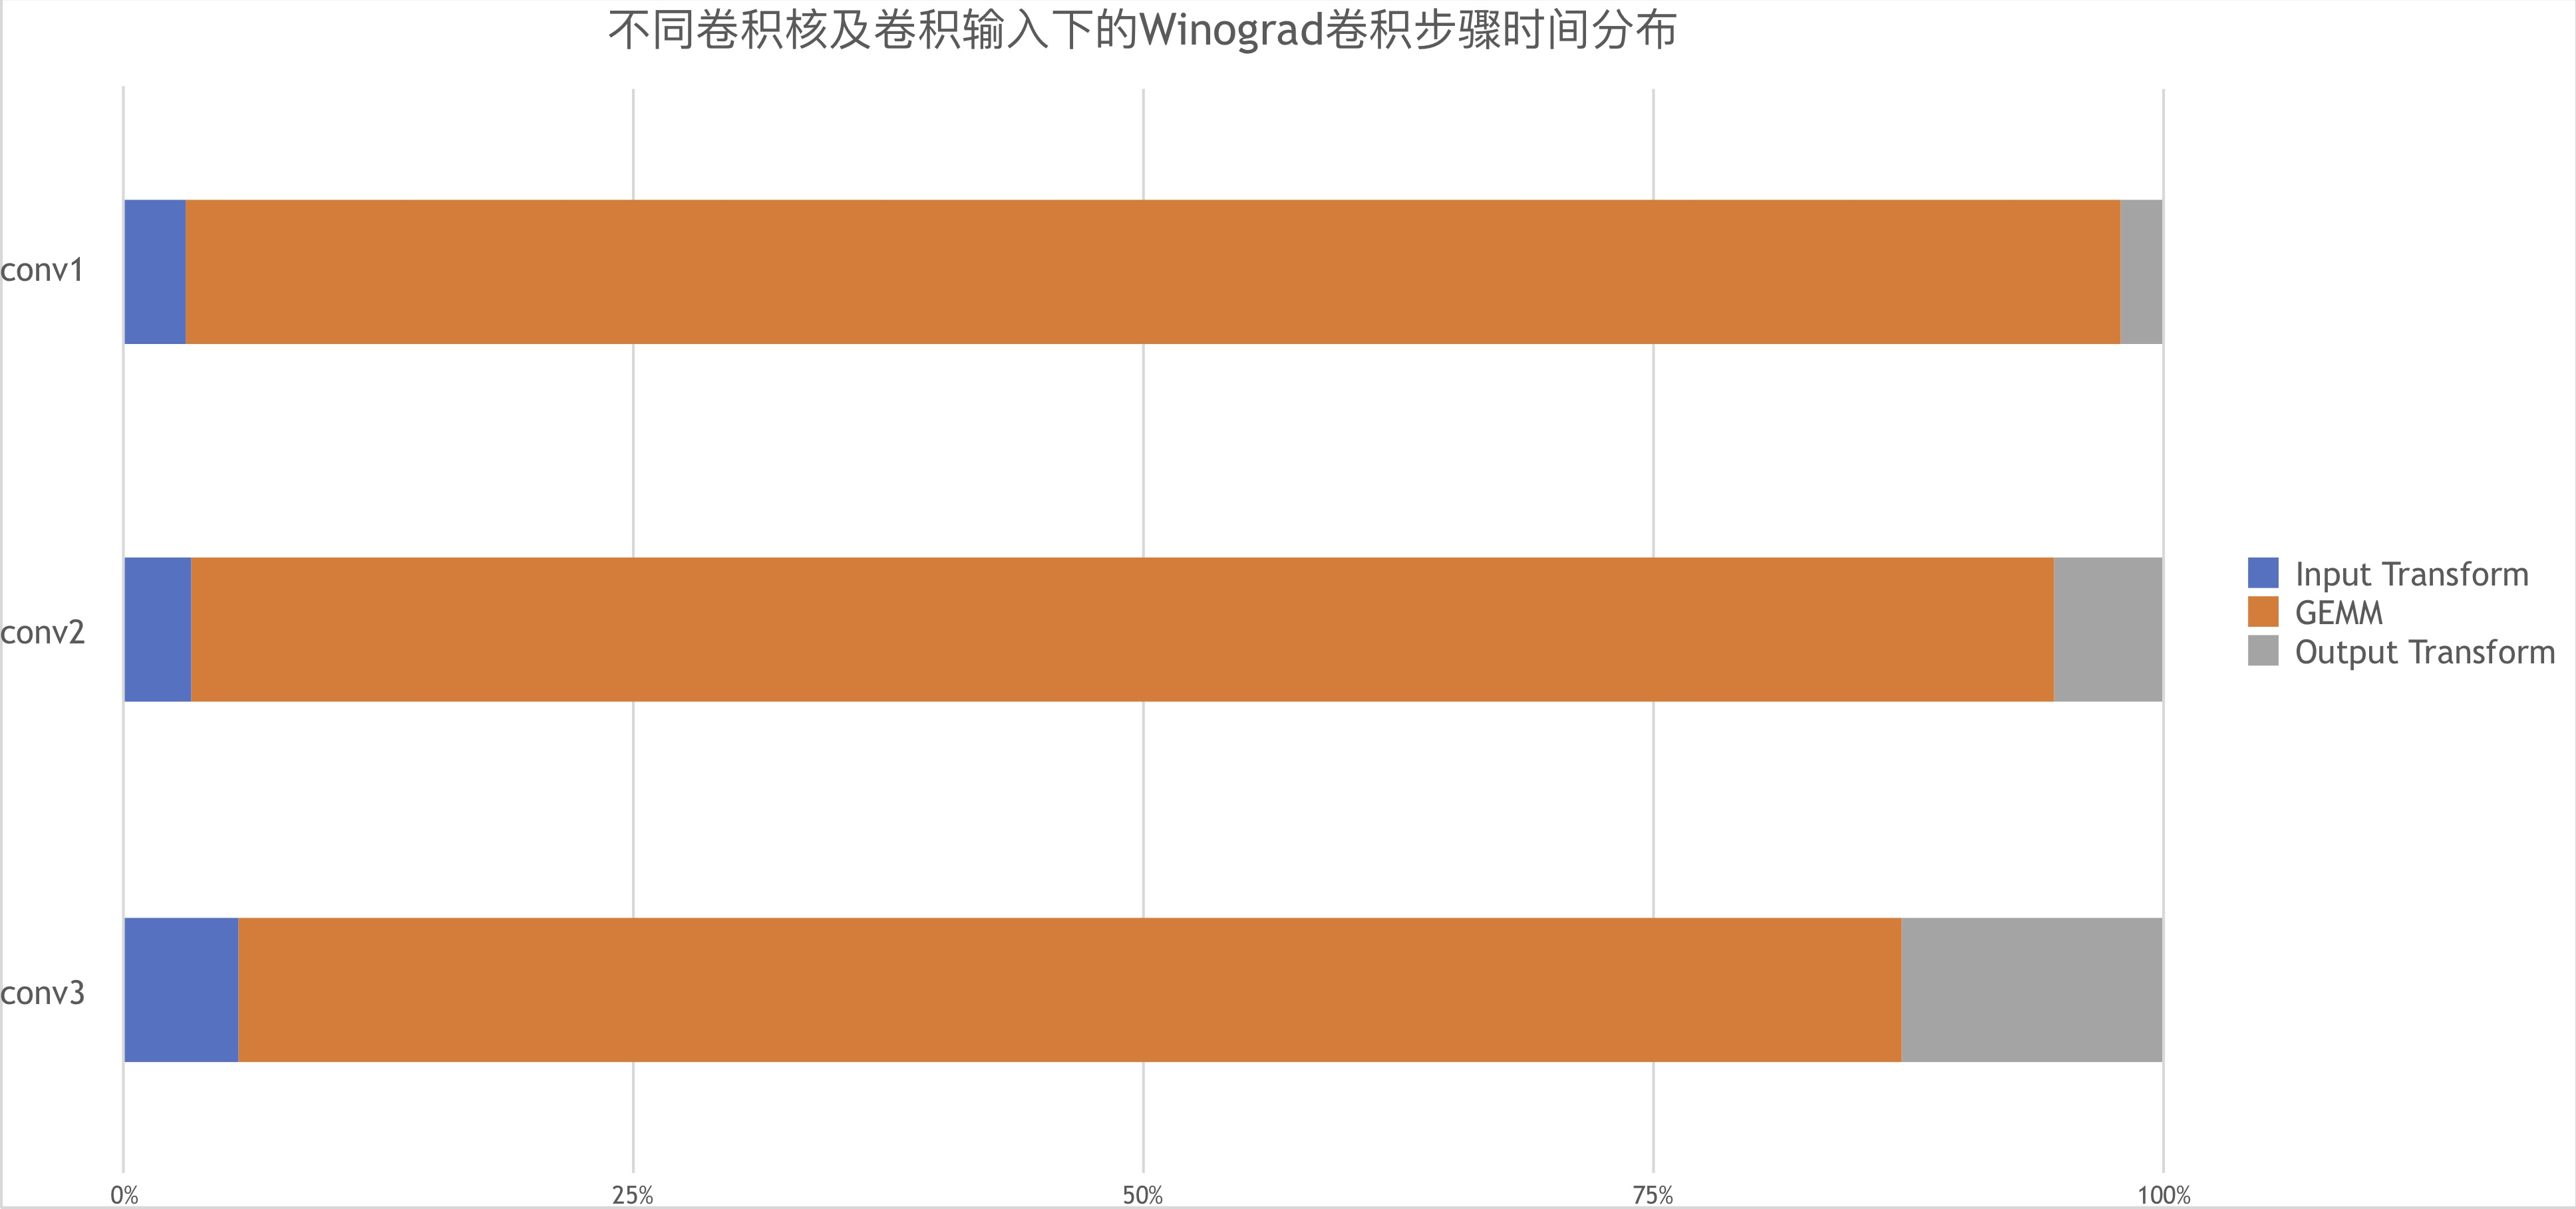
\includegraphics[width=\columnwidth]{wino_conv_dist}
\caption{不同输入及卷积尺度下Winograd 卷积中各个阶段的时间(ms)分布}
\label{fig:wino_conv_dist}
\end{figure}

